%!TEX root=document.tex
\section{Performance Evaluation}
\label{sec:experiments}
 
In the next two sections, we present a thorough evaluation of \SeeDB both in terms
of performance when returning top-$k$ visualizations and in terms of user 
studies.
In this section, we focus on performance studies, where our goal is to evaluate how well our sharing and pruning
optimizations improve latency, and how our pruning optimizations affect accuracy.
%Our goal with the user studies (Section \ref{sec:user_study}), in contrast, is to validate 
%our utility metric by comparing \SeeDB recommendations to ground truth, and to compare 
%\SeeDB to a manual chart construction tool for visual analysis.

In both sections, we report results for \SeeDB on a variety of real and synthetic datasets listed in Table 
\ref{tab:datasets}.
% Our performance studies focus on the synthetic and larger real-world datasets that
% exercise the optimization capabilities of \SeeDB.
% Our user studies, on the other hand, use smaller real-world datasets that are easy to
% understand and where \SeeDB latency 

\begin{table}[htb]
  \centering \scriptsize
  \begin{tabular}{|c|c|c|c|c|c|c|} \hline
  Name & Description & Size & |A| & |M| & Views & Size \\ 
   &  &  &  &  &  & (MB) \\ \hline
  \multicolumn{7}{|c|} {Synthethic Datasets} \\ \hline
  % SYN1 & Synthetic data & 1M & 50 & 5 & 250 \\
  % & Randomly distributed, & & & & \\ 
  % & varying \# distinct values & & & & \\ \hline
  SYN & Synthetic data & 1M & 50 & 20 & 1000 & 411 \\
  & Randomly distributed, & & & & & \\ 
  & varying \# distinct values & & & & & \\ \hline
  SYN*-10 & Synthetic data & 1M & 20 & 1 & 20 & 21\\
  & Randomly distributed, & & & & & \\ 
  & 10 distinct values/dim & & & & & \\ \hline
  SYN*-100 & Synthetic data & 1M & 20 & 1 & 20 & 21\\
  & Randomly distributed, & & & & & \\ 
  & 100 distinct values/dim & & & & & \\ \hline
  \multicolumn{7}{|c|} {Real Datasets} \\ \hline
  BANK  & Customer Loan dataset & 40K & 11 & 7 & 77 & 6.7\\ \hline
  DIAB  & Hospital data & 100K & 11 & 8 & 88 & 23 \\
  & about diabetic patients & & & & & \\ \hline
  AIR & Airline delays dataset & 6M & 12 & 9 & 108 & 974\\ \hline
  AIR10 & Airline dataset & 60M & 12 & 9 & 108 & 9737\\ 
  & scaled 10X & & & & & \\ \hline
  \multicolumn{7}{|c|} {Real Datasets - User Study} \\ \hline
  CENSUS  & Census data & 21K & 10 & 4 & 40 & 2.7\\ \hline
  HOUSING  & Housing prices & 0.5K & 4 & 10 & 40 & $<$1\\ \hline
  MOVIES  & Movie sales & 1K & 8 & 8 & 64 & 1.2\\ \hline
  \end{tabular}
  \vspace{-10pt}
  \caption{Datasets used for testing}
  \label{tab:datasets} 
  \vspace{-10pt}
\end{table}


In each experiment, our primary evaluation metric is latency, i.e., 
how long does it take \SeeDB to return the top-$k$ visualizations. 
For experiments involving our pruning strategies, we measure quality of results through two additional
metrics, namely {\it accuracy} and {\it utility distance} (discussed further in Section 
\ref{sec:custom_execution_engine_expts}).
Since we expect data layout to impact the efficacy of our optimizations, we 
evaluate our techniques on Postgres, a row-oriented database (denoted ROW) as well as Vertica, 
a column-oriented database (denoted COL).

The following experiments use {\it earth mover distance (EMD)} as our distance function for
computing deviation (Section \ref{sec:problem_statement}).
In Section \ref{sec:discussion}, we briefly discuss results of using different distance functions to
compute deviation.
All experiments were run on a single machine with 8 GB RAM and a 16 core Intel 
Xeon E5530 processor. 
Unless described otherwise, experiments were repeated 3 times and the measurements 
were averaged.

We begin by presenting a summary of our experimental findings and then dive into performance results 
for individual optimizations.

%  present the overall results of our applying all our optimizations and then dive into
% performance results for each of our optimizations.
% We begin with a study of the DBMS-backed execution engine and examine how far we can
% push conventional relational engines to support a \SeeDB workload.
% The results motivate empirically the need for our custom execution engine.
% We then present our evaluation of the custom execution engine and pruning strategies.
% The datasets used in our experiments are listed in Table~\ref{tab:datasets}.
% We test our 
% techniques on a variety of syntheic as well as real datasets to evaluate 
% their performance and accuracy.

%!TEX root=document.tex


\subsection{Summary of Findings}
\label{sec:expt_summary}

\reviewer{
	It would be good to investigate the usefulness of the results for queries
with different ranges (for example: if Dq is a very large portion of D, it won’t
have a large deviation from average and thus it is not clear if the
recommended visualizations can be useful)
}

%The previous sections described the basic framework for \SeeDB and our suite of sharing and pruning optimizations.
% two suits of optimizations to efficiently process, we developed a basic framework and sets of pruning an sharing optimizations for \SeeDB.
Figures \ref{fig:all_opt_with_pruning}.a and \ref{fig:all_opt_with_pruning}.b show a summary of \SeeDB performance for the four 
(large) real datasets from Table \ref{tab:datasets} (BANK, DIAB, AIR and AIR10).
For each dataset, we show the latencies obtained on the ROW and COL store by the basic \SeeDB framework (NO\_OPT), 
by our sharing optimizations (SHARING), and by the combination of our sharing and pruning optimizations (COMB). 
We also show latencies for early result generation with COMB (COMB\_EARLY), where we return approximate results 
as soon as the top-$k$ visualizations have been identified.
The results in Figure \ref{fig:all_opt_with_pruning} 
use the CI pruning scheme and $k$=10. We summarize our results below:

%We note that overall the results on the column store (not shown) are similar, with slightly faster overall performance.  The column store benefits less from the pruning optimizations on small datasets (BANK and DIAB), because it has a higher fixed per-query overhead than Postgres, which causes the additional queries run for each round of the pruning algorithm to introduce some penalty.  However, on these datasets the total runtimes are still only a few seconds or less no matter which optimizations we enable.

% (This figure shows results for ROW. Results for COL are discussed further in Section \ref{sec:sharing_and_pruning}).

% \begin{figure}[t]
% 	\centering
% 	\begin{subfigure}{0.24\linewidth}
% 		{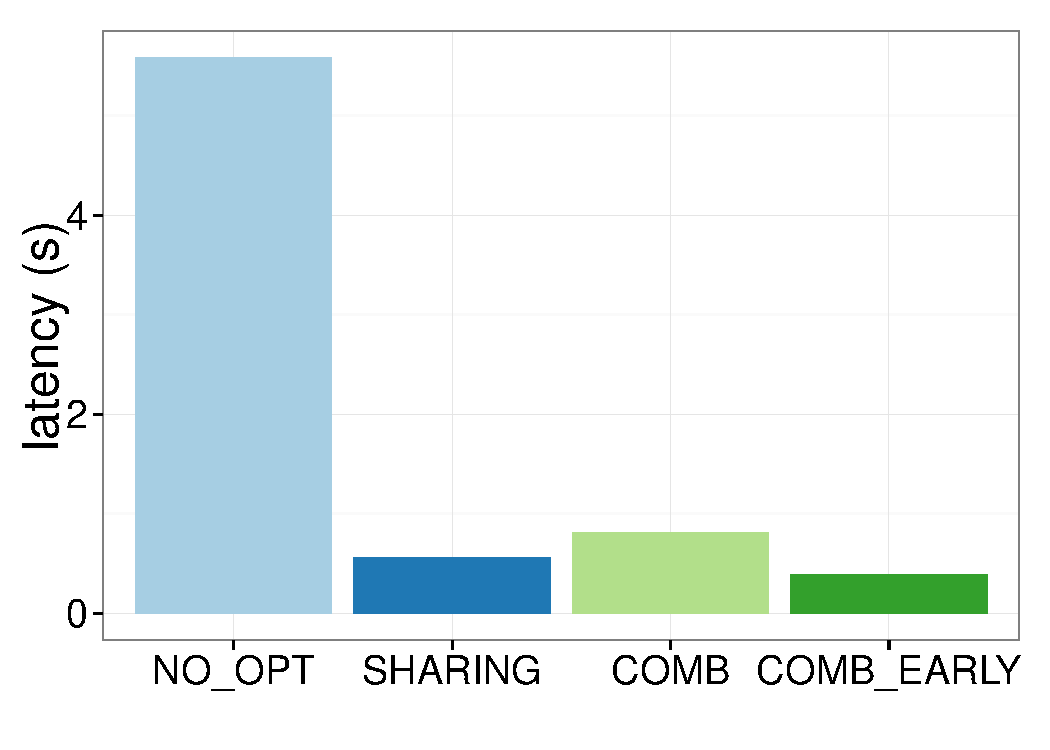
\includegraphics[width=3cm] {Images/all_opt_real_data_row_BANK.pdf}}
% 		\caption{BANK}
% 		\label{fig:baseline_size}
% 	\end{subfigure}
% 	\begin{subfigure}{0.24\linewidth}
% 		\centering
% 		{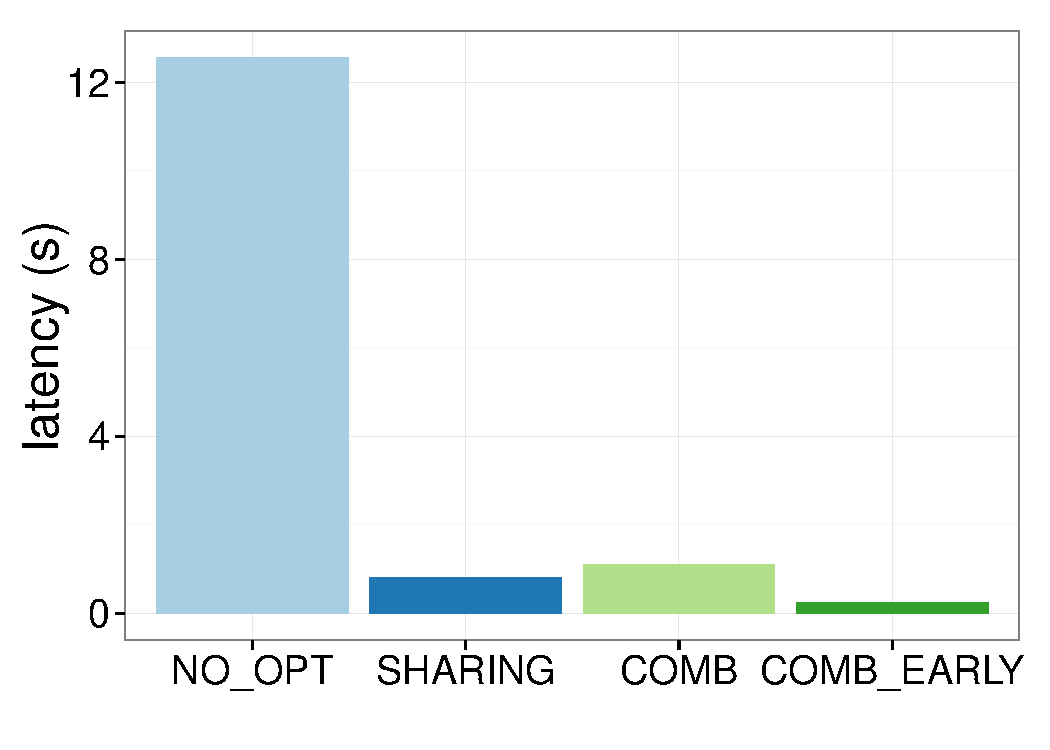
\includegraphics[width=3cm] {Images/all_opt_real_data_row_DIAB.pdf}}
% 		\caption{DIAB}
% 		\label{fig:baseline_views}
% 	\end{subfigure}
% 	\begin{subfigure}{0.24\linewidth}
% 		{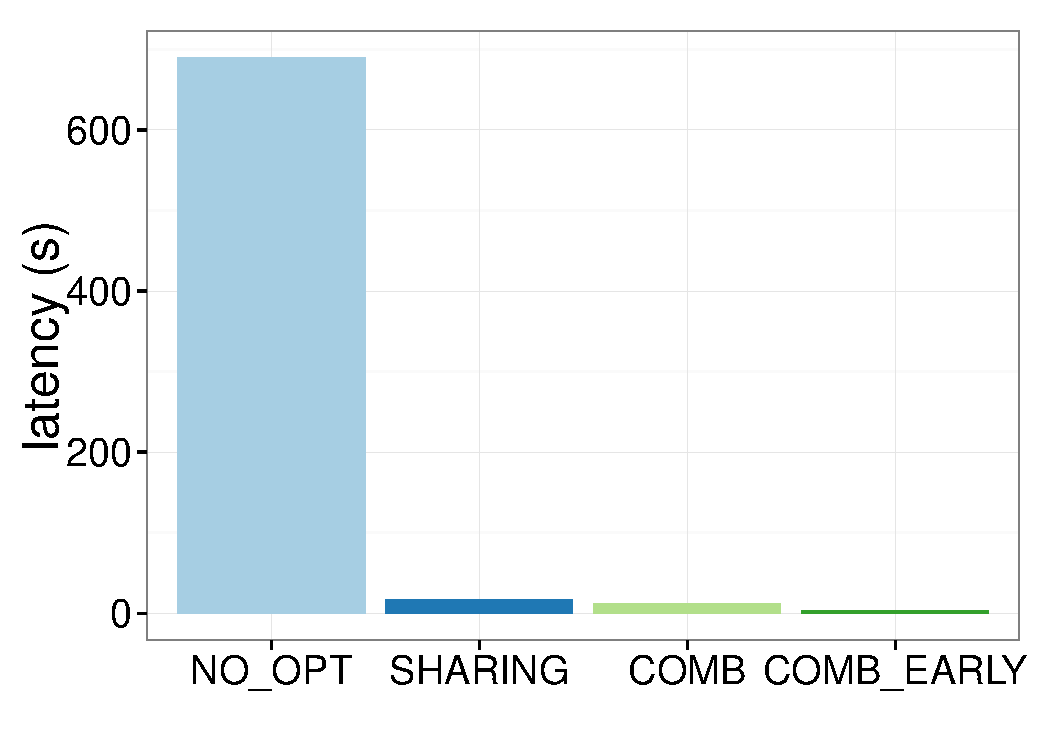
\includegraphics[width=3cm] {Images/all_opt_real_data_row_AIR.pdf}}
% 		\caption{AIR}
% 		\label{fig:multi_agg}
% 	\end{subfigure}
% 	\begin{subfigure}{0.24\linewidth}
% 		{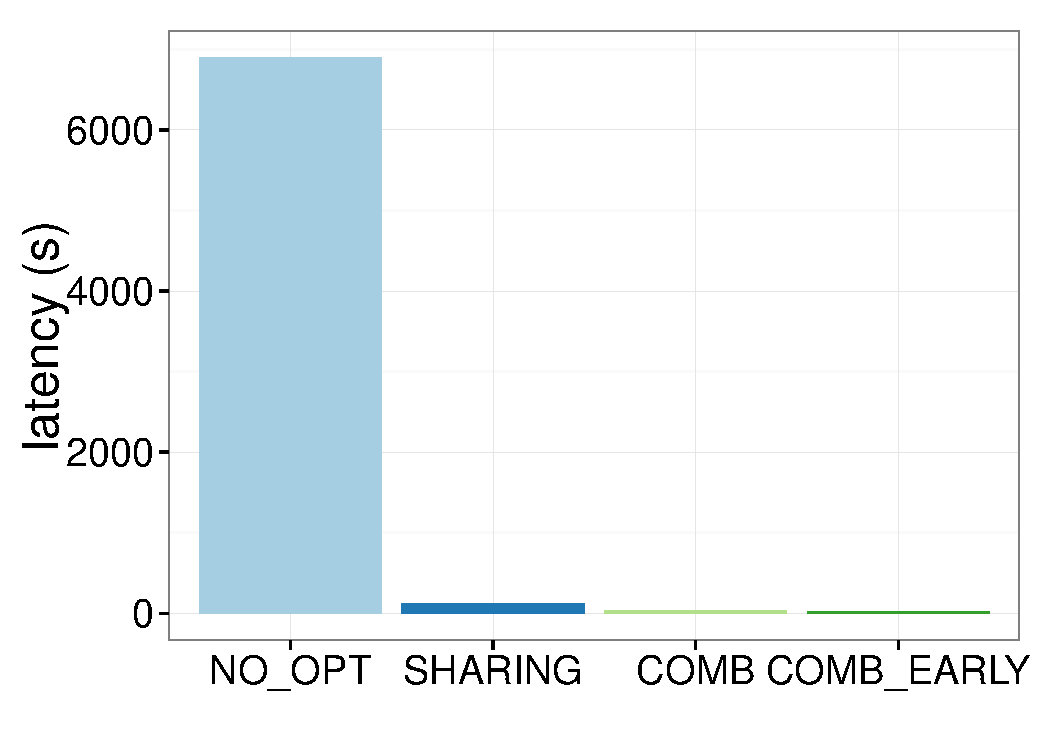
\includegraphics[width=3cm] {Images/all_opt_real_data_row_AIR10.pdf}}
% 		\caption{AIR10}
% 		\label{fig:multi_agg}
% 	\end{subfigure}
% 	\vspace{-10pt}
% 	\caption{Performance gains of all optimizations in ROW }
% 	\vspace{-10pt}
% 	\label{fig:share_prune_row}
% \end{figure}

% \begin{figure*}[t]
% 	\centering
% 	\begin{subfigure}{0.33\linewidth}
% 		\centering
% 		{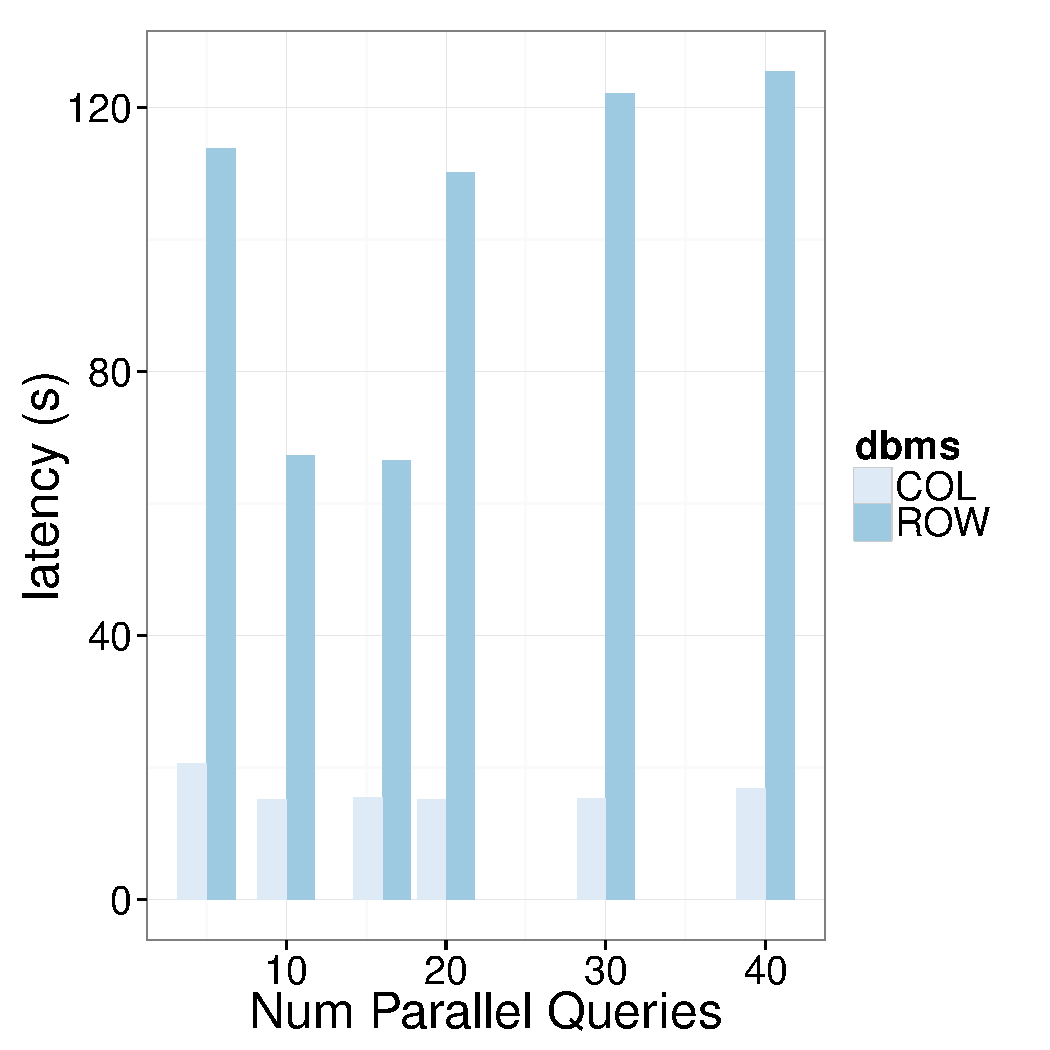
\includegraphics[width=6cm] {Images/parallel_noop.pdf}}
% 		\caption{Effect of parallelism}
% 		\label{fig:parallelism}
% 	\end{subfigure}
% 	\begin{subfigure}{0.33\linewidth}
% 		\centering
% 		{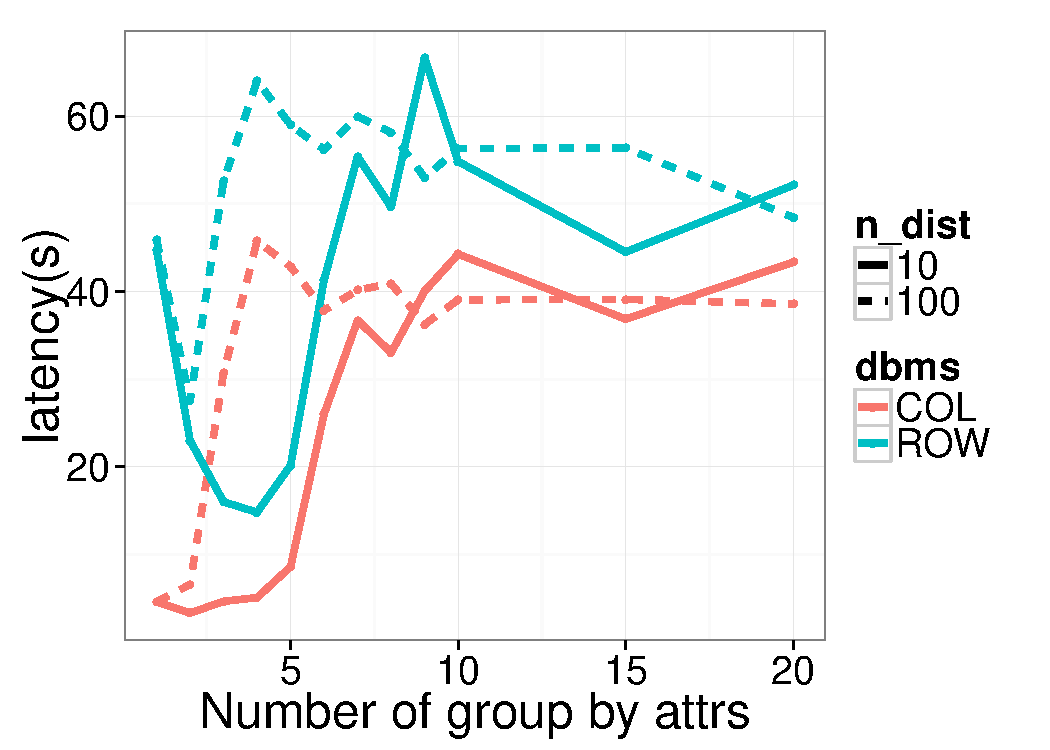
\includegraphics[width=6cm] {Images/multi_gb_same.pdf}}
% 		\caption{Latency vs. Num of Groups}
% 		\label{fig:multi_gb_same}
% 	\end{subfigure}
% 	\begin{subfigure}{0.33\linewidth}
% 		\centering
% 		{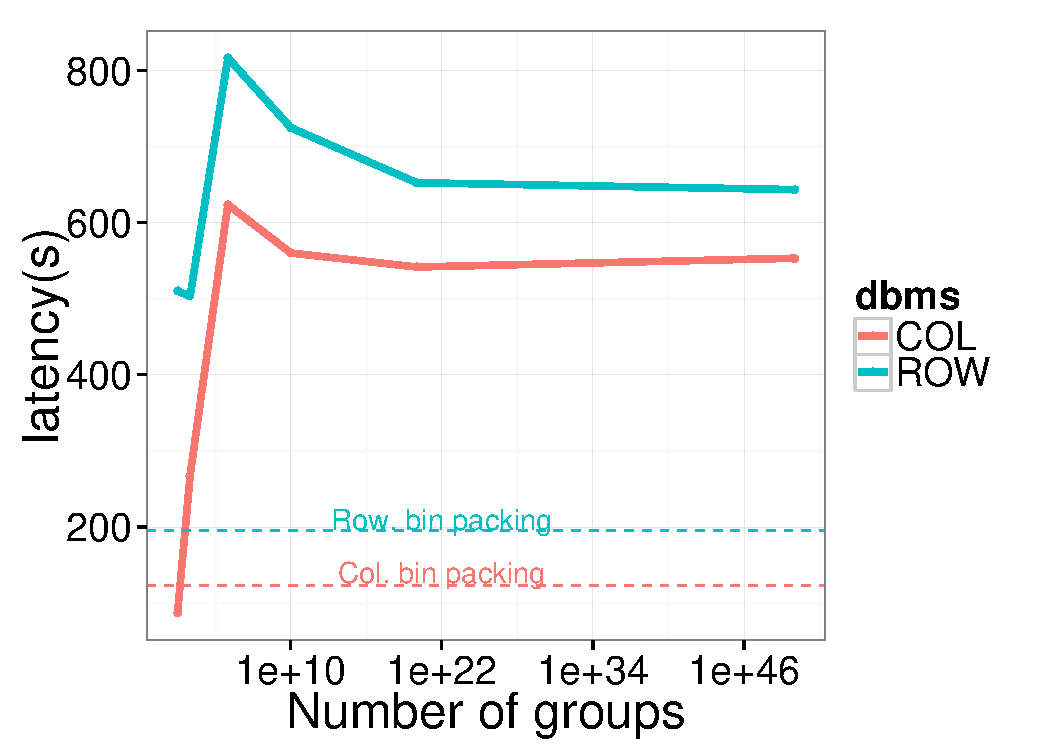
\includegraphics[width=6cm] {Images/multi_gb.pdf}}
% 		\caption{Latency vs. Num Dimensions}
% 		\label{fig:multi_gb_bp}
% 	\end{subfigure}
% 	\vspace{-10pt}
	
% 	\label{fig:bank_perf}
% 	\vspace{-10pt}
% \end{figure*}

\begin{figure}[h]
\vspace{-5pt}
	\centering
	\begin{subfigure}{1\linewidth}
		\centering
		{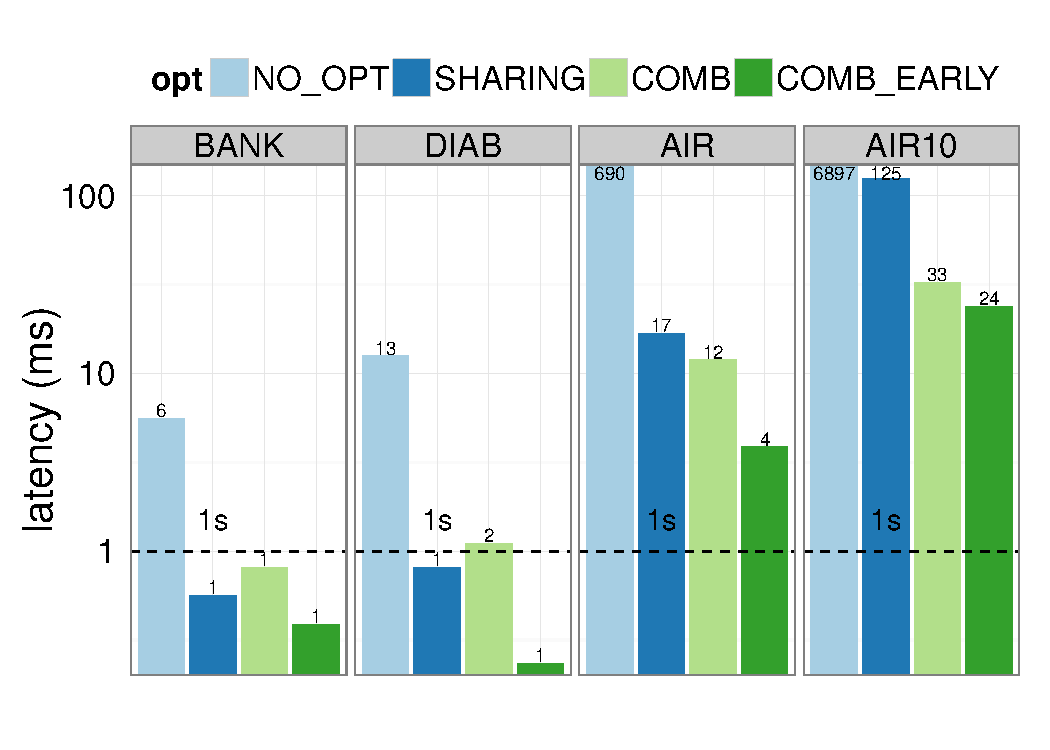
\includegraphics[width=7cm] {Images/all_opt_real_data_row.pdf}}
		\vspace{-15pt}
		\caption{Optimization results for ROW}
		\label{fig:share_prune_row}
	\end{subfigure}\\
	\begin{subfigure}{1\linewidth}
		\centering
		{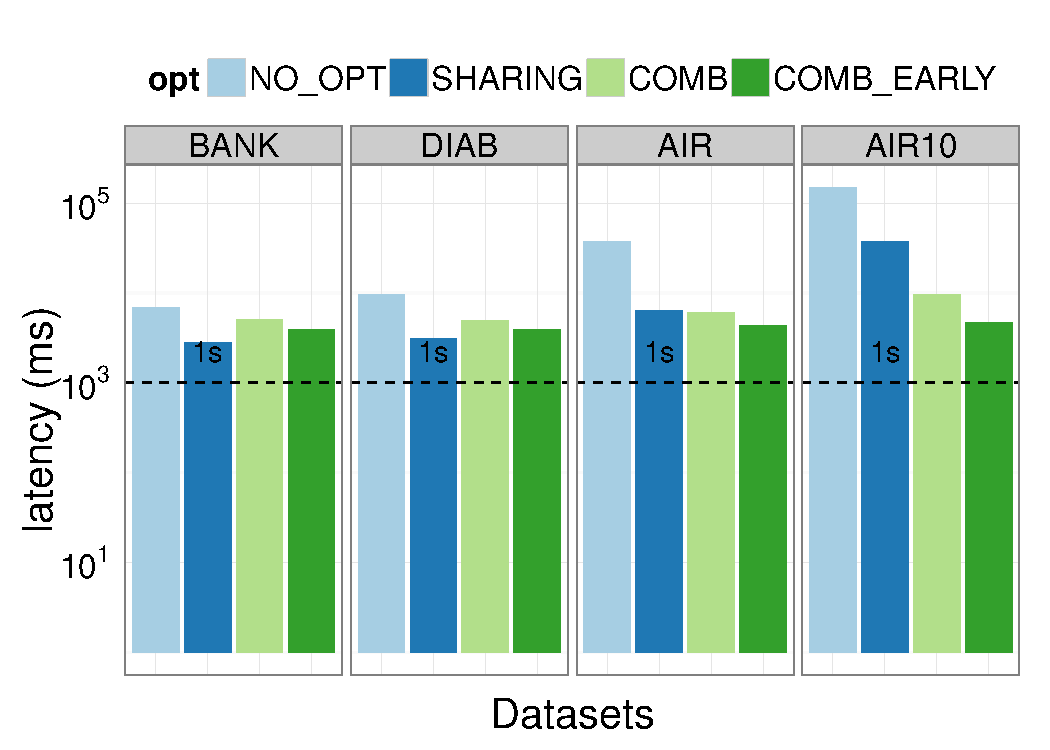
\includegraphics[width=7cm] {Images/all_opt_real_data_col.pdf}}
		\vspace{-15pt}
		\caption{Optimization results for COL}
		\label{fig:share_prune_col}
	\end{subfigure}
	\vspace{-10pt}
	\caption{Performance gains from all optimizations}
	\label{fig:all_opt_with_pruning}
	\vspace{-15pt}
\end{figure}
 
\begin{denselist} 
\item $[$\underline{\em $>$ 100X speedup overall}$]$ The combination of our sharing and pruning optimizations provides a speedup of up 
between 50X (COMB) -- 300X (COMB\_EARLY) for ROW (Figure \ref{fig:share_prune_row}) and 
10X (COMB) -- 30X (COMB\_EARLY) for COL (Figure \ref{fig:share_prune_col}).
This reduces latencies for small datasets like DIAB from 12s to 200ms, and from almost 2 hrs to tens of seconds for large datasets 
like AIR10. 
{\it Our optimizations thus allows us to respond in real-time with exact views for small datasets and approximate views (COMB\_EARLY) for large datasets}.
\item $[$\underline{\em 8--20X speedup from sharing}$]$ The sharing optimizations (Section \ref{sec:sharing_opt}) alone produce performance gains of up to 20X for ROW and 8X for COL. This enables \SeeDB to process moderate sized datasets within a few seconds.
In fact, for small datasets like BANK and DIAB, the overheads associated with phased-execution can be avoided completely since SHARING
alone can achieve interactive latencies.
\item $[$\underline{\em 5X speedup from pruning without loss of accuracy}$]$ Pruning optimizations (Section \ref{sec:pruning_opt}) provide additional gains of up to 5X. Early result return, in particular, enables real-time response for large datasets, e.g. for AIR, the COMB\_EARLY strategy allows \SeeDB to return results in under 4s while processing the full dataset takes tens of seconds. We also find that quality of results is not adversely affected by pruning: the utility distance (defined later) for our pruning strategies is close to 0.
\item $[$\underline{\em Multiplicative gains}$]$ The {\it gains produced by sharing-based and pruning-based optimizations are multiplicative}. Therefore, a gain of 20X from sharing optimizations in the ROW store combines with the 5X gain from pruning to produce an overall gain of over 100X (Figure \ref{fig:share_prune_row}).
\item $[$\underline{\em Column stores perform better}$]$ In general, COL stores are better suited to the \SeeDB workload and 
significantly outperform ROW stores. The column-oriented data layout of COL enables the selective processing of specific attributes involved in each visualization. 
\item $[$\underline{\em Gains improve on larger datasets}$]$ Finally, while our techniques show performance gains across the board, they are particularly useful for large datasets, e.g. overall gain is much larger for AIR10 (300X) vs. BANK (10X). We find that our SHARING optimization is best suited for small datasets like BANK and DIAB, while COMB and COMB\_EARLY are essential for large datasets like AIR and AIR10.
\end{denselist}


% Thus, we conclude that the COMB and COMB\_EARLY optimizations are best suited for large datasets like AIR and AIR10 while SHARING is suitable for small datasets. 

In the next sections, we discuss the performance of individual optimizations and how they relate to the overall performance gain.




\subsection{DBMS-backed Execution Engine}
\label{sec:expts_dbms_execution_engine}

Our primary metric for evaluating the DBMS-backed
execution engine is {\em latency},
i.e., .
Specifically, we study the impact of the following properties on latency:
(a) parameters of the dataset including size and number of views.
(b) the optimizations detailed in Section~\ref{sec:dbms_optimizations}, and
(c) 
% Our goal is to identify which data layout is a better
% fit for \SeeDB, and study the gains of each optimization
% for row-stores vs.~column stores. 
The following experiments focus on synthetic datasets SYN and SYN* 
(Table~\ref{tab:datasets}) since we can control all parameters of the 
data including size, number of 
attributes, and data distribution.
The performance on the real datasets is similar and hence omitted.
Unless described otherwise, experiments were repeated 3 times and the latency measures 
were averaged.

\begin{figure*}[t]
	\centering
	\begin{subfigure}{0.33\linewidth}
		{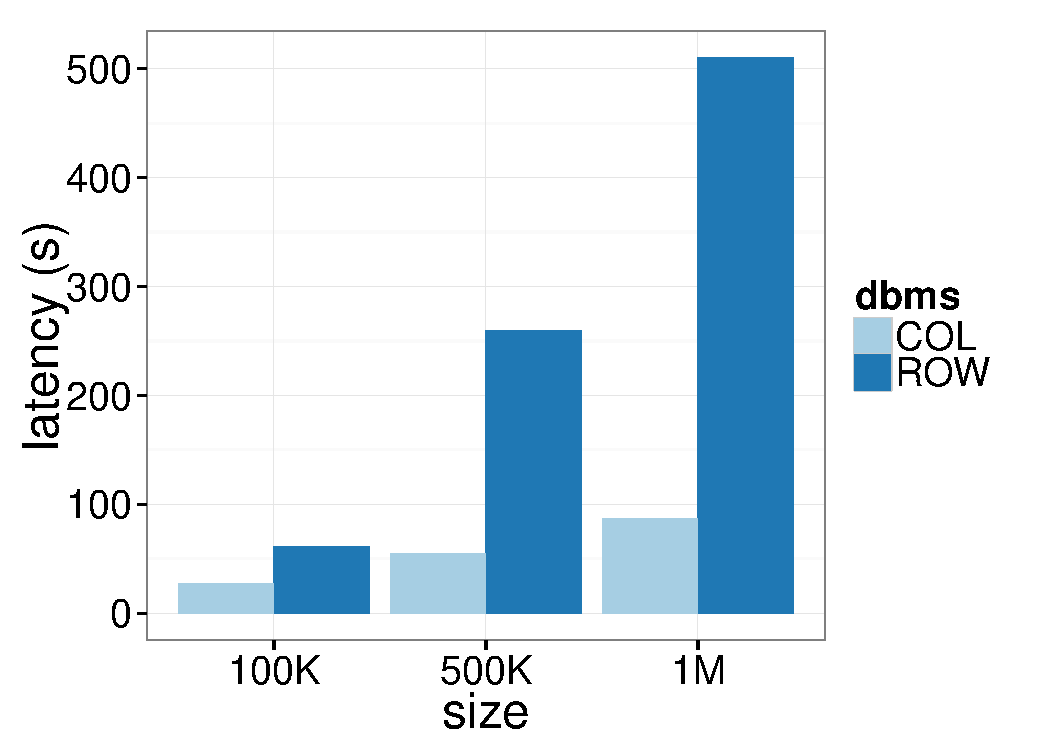
\includegraphics[width=6cm] {Images/baselines_by_size.pdf}}
		\caption{Latency vs. Table size}
		\label{fig:baseline_size}
	\end{subfigure}
	\begin{subfigure}{0.33\linewidth}
		\centering
		{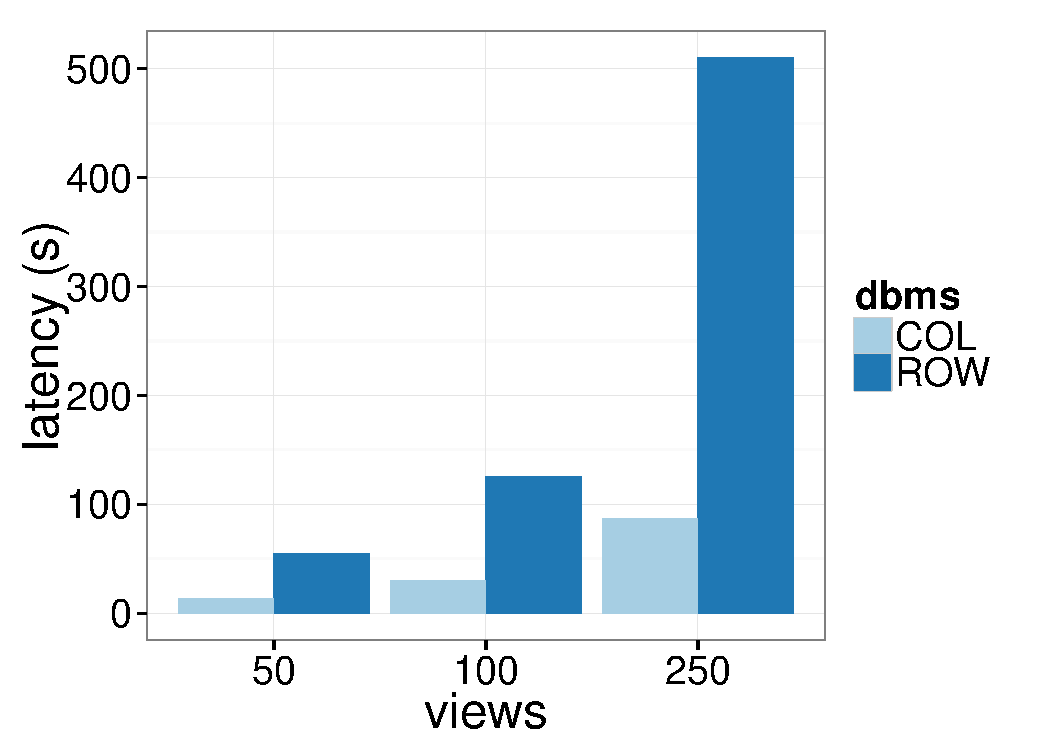
\includegraphics[width=6cm] {Images/baselines_by_views.pdf}}
		\caption{Latency vs. Num Views}
		\label{fig:baseline_views}
	\end{subfigure}
	\begin{subfigure}{0.33\linewidth}
		{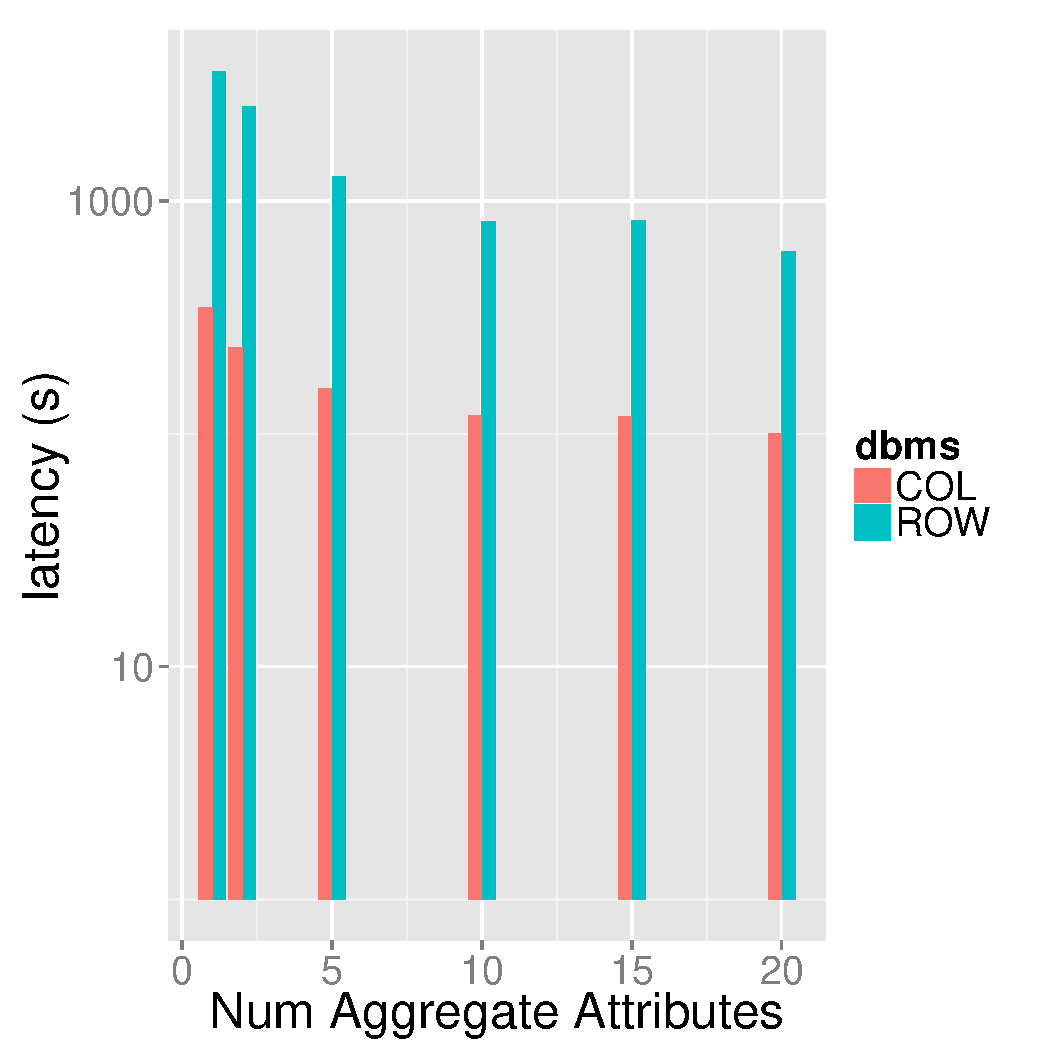
\includegraphics[width=6cm] {Images/multi_agg.pdf}}
		\caption{Latency vs. number of aggregates}
		\label{fig:multi_agg}
	\end{subfigure}
	\vspace{-10pt}
	\caption{Baseline performance and Effect of Combining Aggregates }
	\vspace{-10pt}
	\label{fig:bank_perf}
\end{figure*}

\begin{figure*}[t]
	\centering
	\begin{subfigure}{0.33\linewidth}
		\centering
		{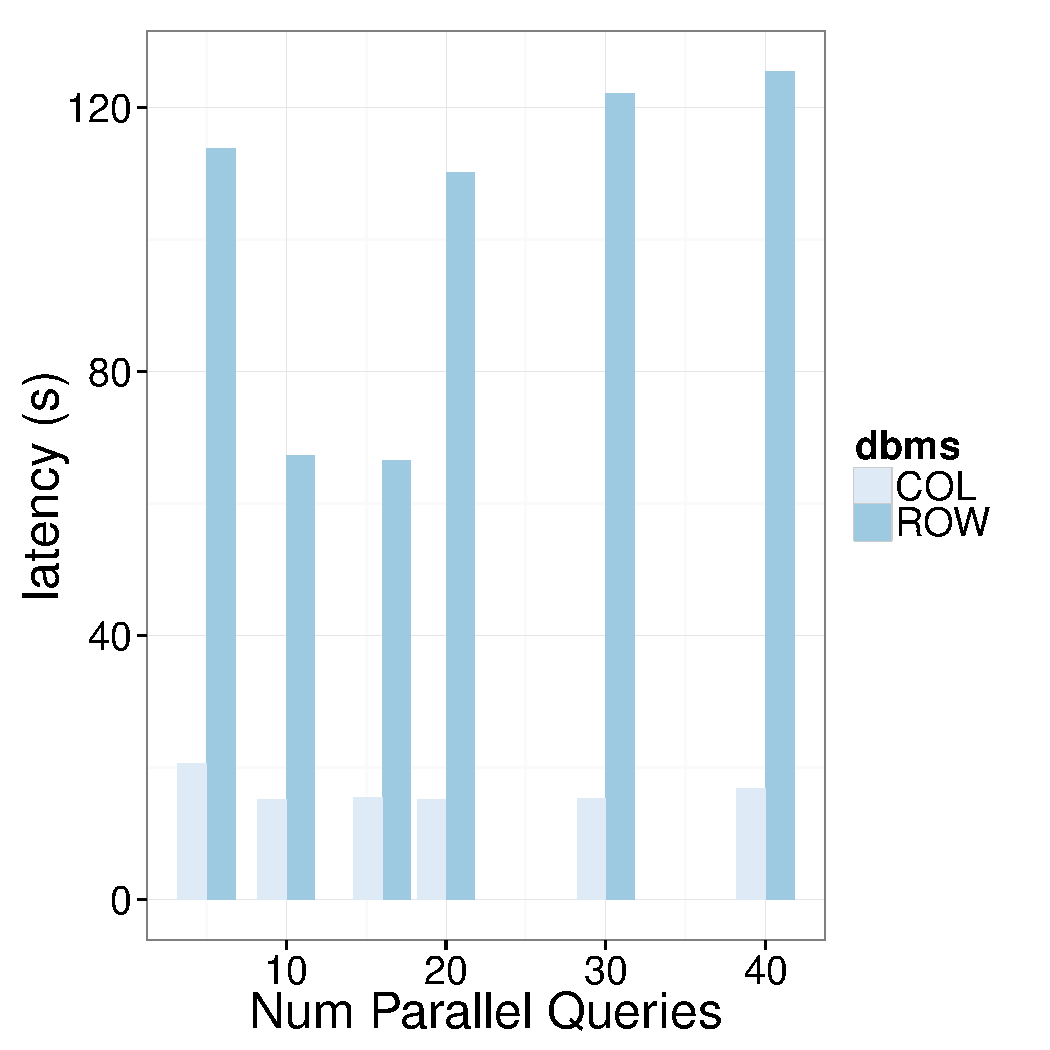
\includegraphics[width=6cm] {Images/parallel_noop.pdf}}
		\caption{Effect of parallelism}
		\label{fig:parallelism}
	\end{subfigure}
	\begin{subfigure}{0.33\linewidth}
		\centering
		{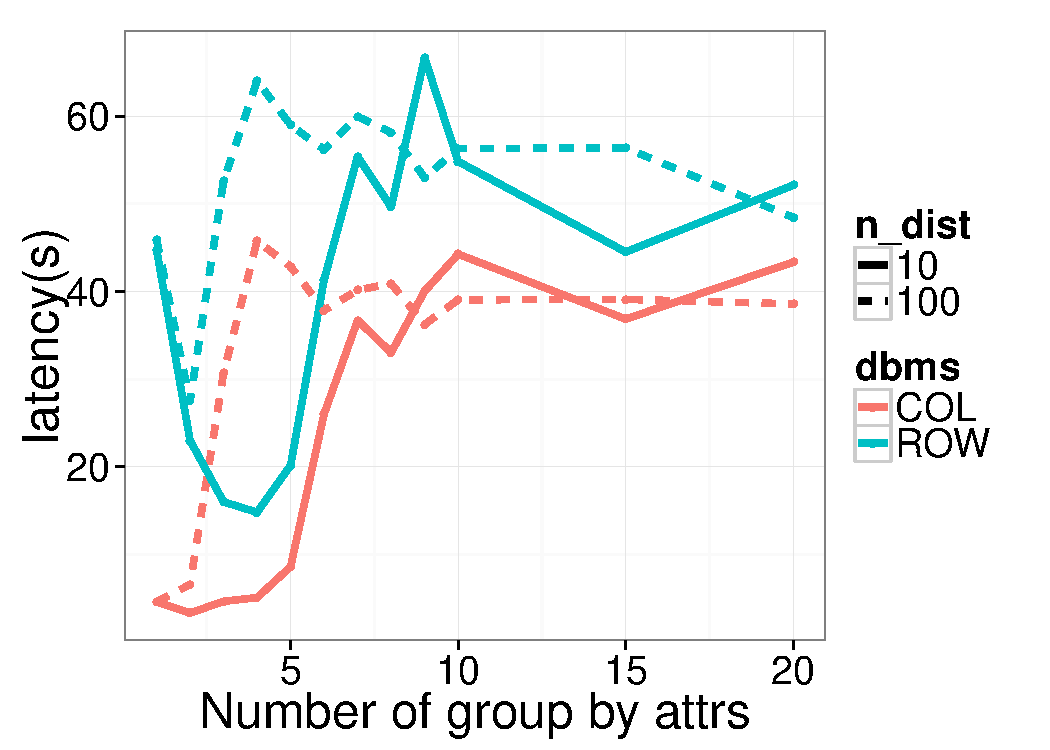
\includegraphics[width=6cm] {Images/multi_gb_same.pdf}}
		\caption{Latency vs. Num of Groups}
		\label{fig:multi_gb_same}
	\end{subfigure}
	\begin{subfigure}{0.33\linewidth}
		\centering
		{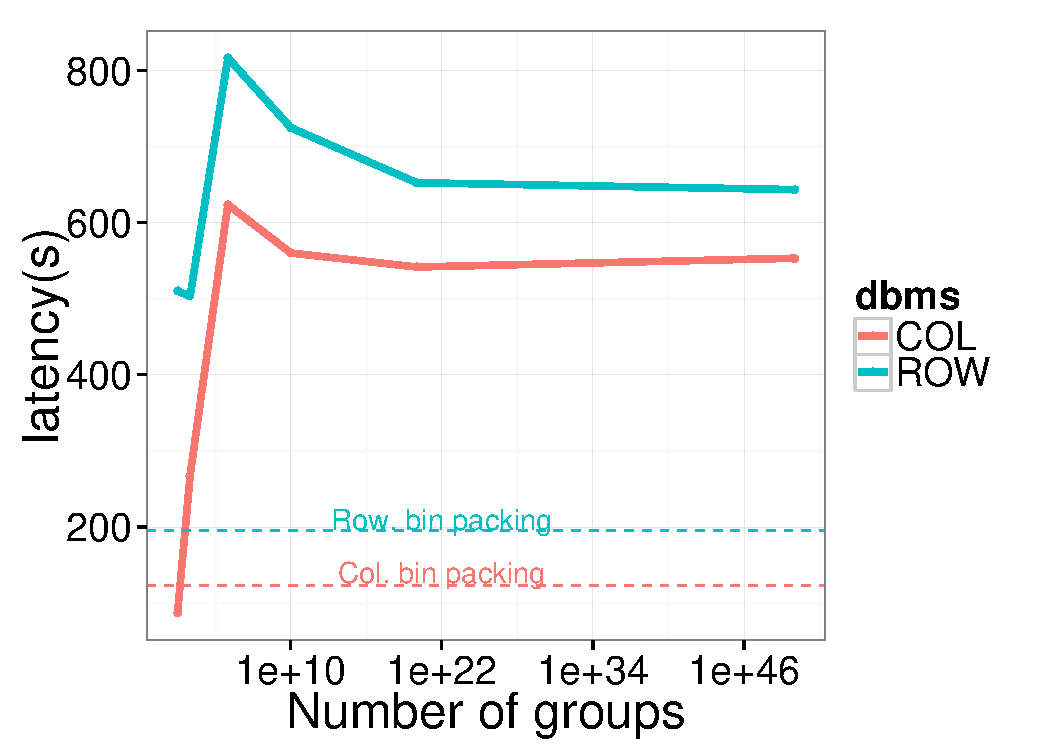
\includegraphics[width=6cm] {Images/multi_gb.pdf}}
		\caption{Latency vs. Num Dimensions}
		\label{fig:multi_gb_bp}
	\end{subfigure}
	\vspace{-10pt}
	\caption{Effect of Combining Group-by attributes and Parallel Query Execution}
	\label{fig:bank_perf}
	\vspace{-10pt}
\end{figure*}


\stitle{Result Highlights:}
\begin{denselist}
\item Our optimizations to the DBMS-based execution engine can reduce
latency on large datasets from 500 seconds (ROW) and 100 seconds (COL)
to about 10 seconds for COL, and about 20 seconds for ROW.
% This is particularly noteworthy given that
% \SeeDB is running 100s of queries on the DBMS for each \SeeDB query.

\item Latency scales linearly 
with dataset size and number of views.

\item Column stores are superior to row stores 
for our workload. Row stores, however, benefit more from the
proposed optimizations. 
% For instance, row stores benefit
% significantly (with reductions of up to 2.5X on latency) from applying
% bin-packing-based algorithms for aggregation, 
% while column stores are not significantly affected. 

\item Although our optimizations lead to a 8X-20X speedup, the total latency remains in the 10s of seconds.
 % - a number unacceptable in interactive systems.
In addition, each \SeeDB query translates to 50+ SQL queries. 
This {\it query bloat} unnecessarily consumes DBMS resources including memory and CPU.
Consequently, we see the need for a custom solution with  lower latencies and a
smaller resource footprint.
\end{denselist}

% As mentioned in Section \ref{sec:dbms_execution_engine}, our DBMS-based
% execution engine leverages the DBMS API to execute view queries directly on the
% database.
% While this approach has the advantages of reusing existing query procesing
% systems and being agnostic to the specific underlying DBMS, its limitations
% include the lack of fine grained control over sharing of table scans and lack of
% ability to prune low-utility views. 

We start with an evaluation of the basic framework (without any optimizations) 
and then study the effect of the proposed optimizations (Section~\ref{sec:dbms_optimizations}).
% Our goal is to characterize the effect of each optimization and find the optimal parameter 
% settings for the DBMS execution engine.
% , i.e., 
% how long do row and column stores take if each view is evaluated 
% in sequence, without any optimization. 
% We then study the effect of adding each optimization from Section~\ref{sec:dbms_optimizations} 
% in turn.

\stitle{Basic No Optimization Framework:} 
{\em \underline{Summary:} Applying no optimizations 
leads to latencies in the 100s of seconds for both ROW and COL;
latency increases linearly in the size of the dataset and  number
of views. 
Column stores are superior to row stores,
with $\frac{1}{5}$th the latency.}
Without any optimizations, the basic DBMS-backed execution engine
serially executes individual view queries, two for each possible view.
Figure \ref{fig:baseline_size} shows latency of \SeeDB\ vs. the number of rows (100K rows--1M rows) in the dataset while  
Figure \ref{fig:baseline_views} shows latency as a function 
of the number of views (50--250).
These experiments were run on the SYN dataset by varying the size of the
table and number of attributes.
% and we created subsets of the dataset with
% varying numbers of rows and views, by varying the number of dimension attributes. 
First, notice that the basic no optimization framework has very 
poor performance: latency for ROW is between 50-500s, 
while it is between 10-100s for COL. 
This is because both ROW and COL run 50 to 250 SQL queries for each \SeeDB query.
These time scales are not practical for interactive applications. 
Second, COL runs about 5X faster than ROW. 
This is expected because individual view queries only select one dimension
attribute and one measure attribute at a time.  
COL can just read these two
columns, whereas ROW must read all columns.
Third, as expected, the latency of the
basic framework is proportional to the number of rows as well as the 
number of views in the table.
Since the latencies for the basic framework are very high for interactive
applications, it is clear that aggressive optimization needs to be employed. 

% \begin{figure}[h] 
% \centerline{
% \resizebox{4cm}{!} {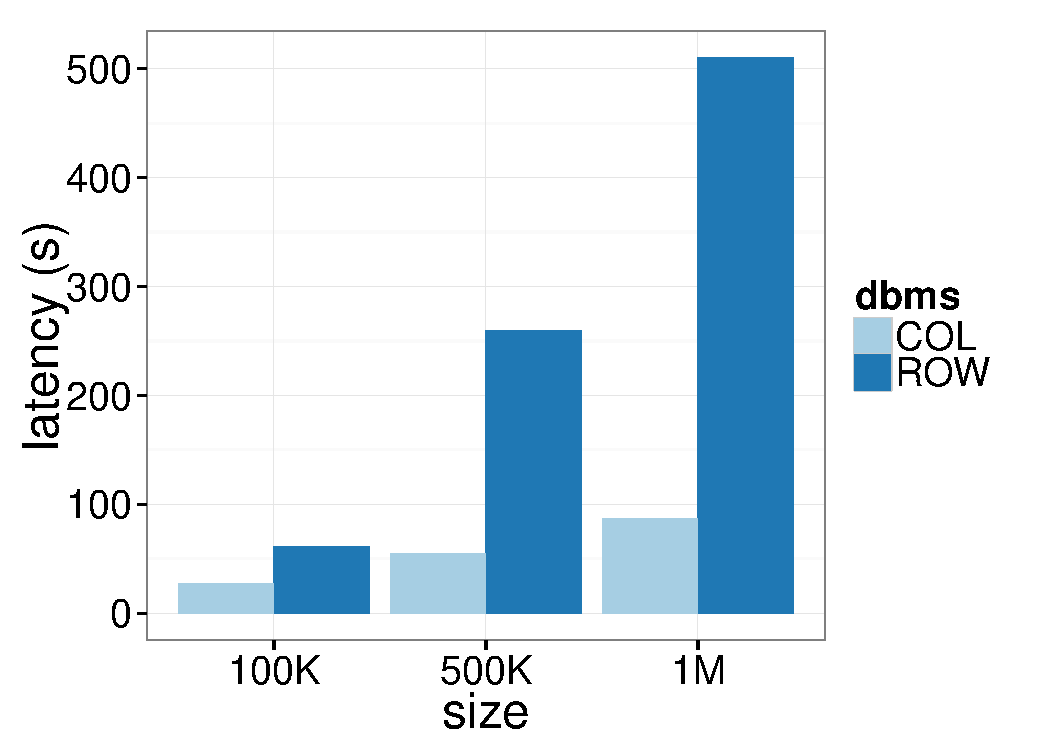
\includegraphics {Images/baselines_by_size.pdf}}
% \resizebox{4cm}{!} {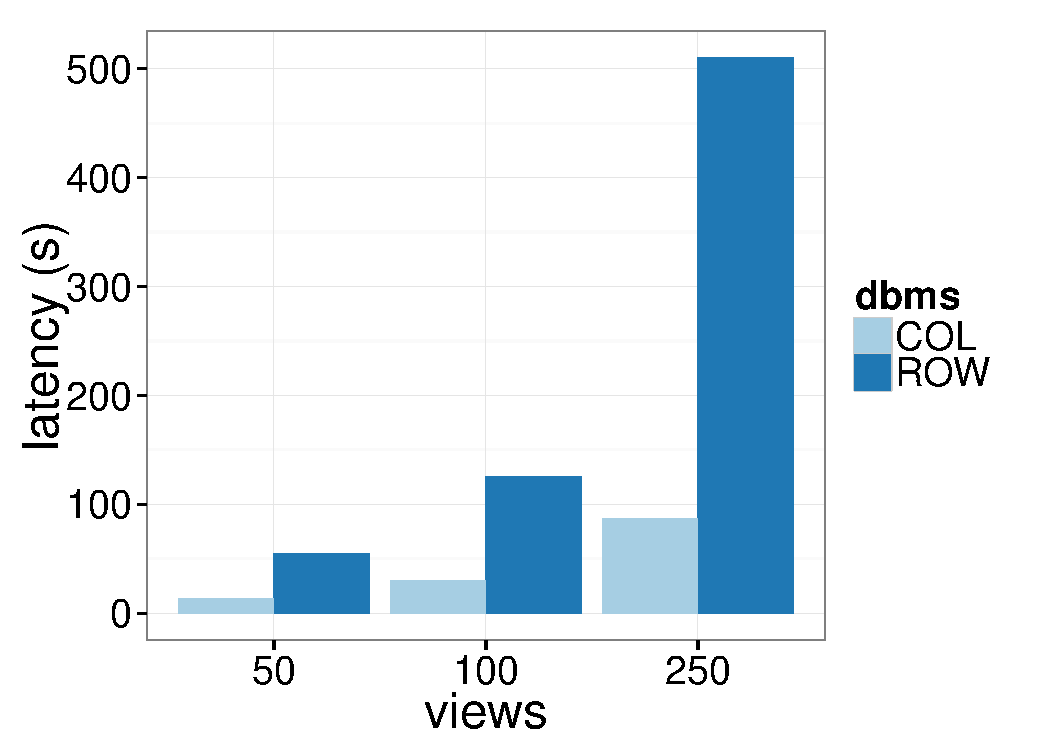
\includegraphics {Images/baselines_by_views.pdf}}
% }
% \end{figure}



% \begin{figure}[h]
% \centering
% \begin{subfigure}{0.49\linewidth}
% \centering
% {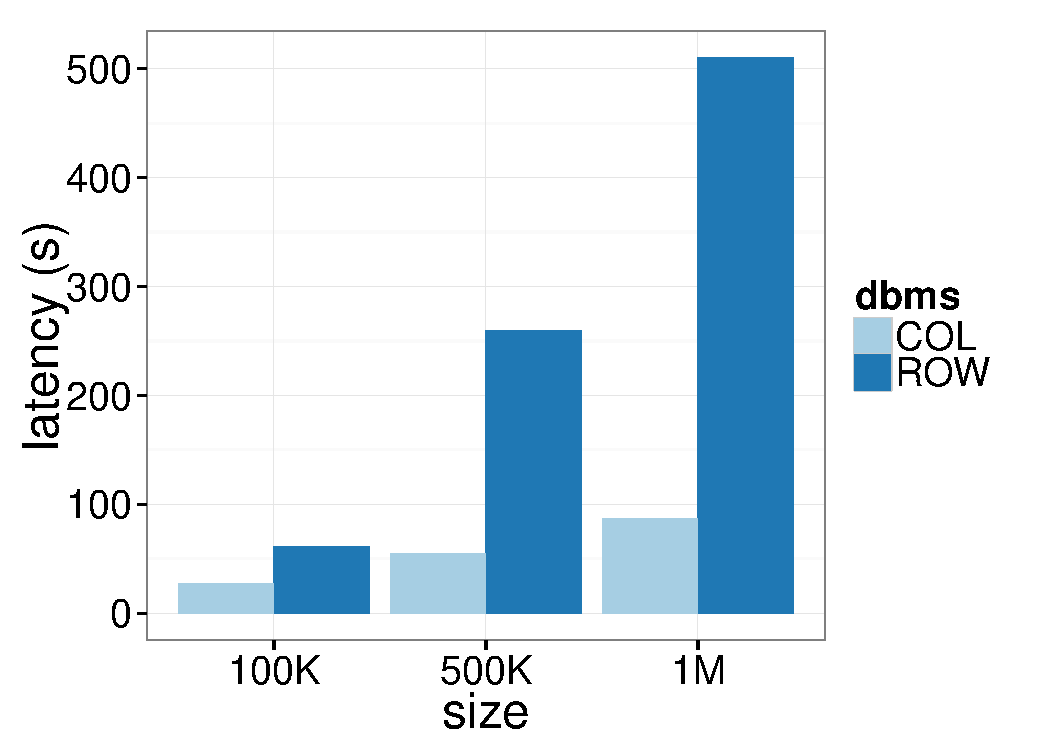
\includegraphics[width=4.2cm] {Images/baselines_by_size.pdf}}
% \caption{Latency vs. Table size}
% \label{fig:baseline_size}
% \end{subfigure}
% \begin{subfigure}{0.49\linewidth}
% \centering
% {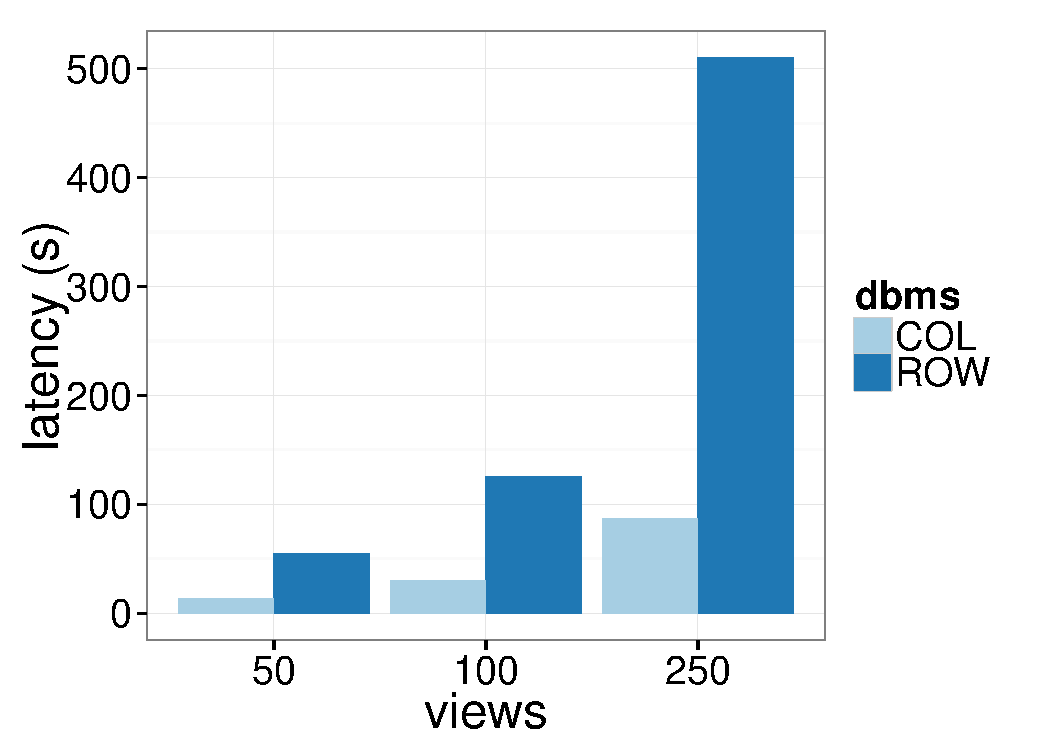
\includegraphics[width=4.2cm] {Images/baselines_by_views.pdf}}
% \caption{Latency vs. Num Views}
% \label{fig:baseline_views}
% \end{subfigure}
% \label{fig:baselines}
% \caption{Latency of Basic Framework}
% \end{figure}

\stitle{Combining Multiple Aggregates:} 
{\em \underline{Summary:} Combining view queries with the same group-by attribute
but different aggregates gives a 
3-4X speedup for both row and column stores.}
To study the limits of adding multiple aggregates to a single query, we ran \SeeDB
by varying the limit on the number of aggregates in any generated SQL query 
($n_{agg}$) between 1 and 20.
% We combine multiple view queries that have the same group-by (dimension) 
% attribute, but different aggregation (measure) attributes into one query.
% We ran these experiments on the SYN2 dataset 
% since it has a large number (20) of measure attributes.
% We varied the number of aggregate attributes 
% in a query between 1 and 20 (i.e., we grouped $n_{agg}$ view
% queries that share the same group-by attribute into one query
% that is issued to the DBMS).
The resulting latencies on the SYN dataset are shown in Figure \ref{fig:multi_agg} (log scale on the y-axis).
As we can see, latency reduces consistently with the number of aggregations performed 
per query.
The latency reduction is however not linear in $n_{agg}$ because
larger $n_{agg}$ values require maintenance of more state and access of more columns in a 
column store.
Overall, we get a 4X speedup for row stores and a 3X speed up for column stores.

\stitle{Parallel Query Execution:} 
{\em \underline{Summary:} Running view queries in parallel can offer significant
performance gains; however, there is an optimal number of parallel queries
beyond which performance degrades significantly.}
Executing \SeeDB-generated SQL queries in parallel can provide significant performance gains
because queries can share buffer pool pages.
However, a high degree of parallelism can degrade performance for a variety of reasons \cite{Postgres_wiki}. 
Figure \ref{fig:parallelism} illustrates this issue: we varied the maximum number of parallel queries
issued by \SeeDB and measured the resulting latency.
As expected, low levels of parallelism produced sizable performance gains but
high levels led to degraded performance.
For both row and column stores in our system, the optimal number of queries to 
run in parallel is approximately $16$ (equal to the number of cores). 
% This appears to hold true for both row or column stores. 
In general, we have found that choosing a degree of parallelism equal to the number of cores
% for these kinds of simple aggregation queries when data largely fits in memory,
is a reasonable rule of thumb. 
% \mpv{separate this from general study of parallel queries}

% \begin{figure}[h]
% \centering
% {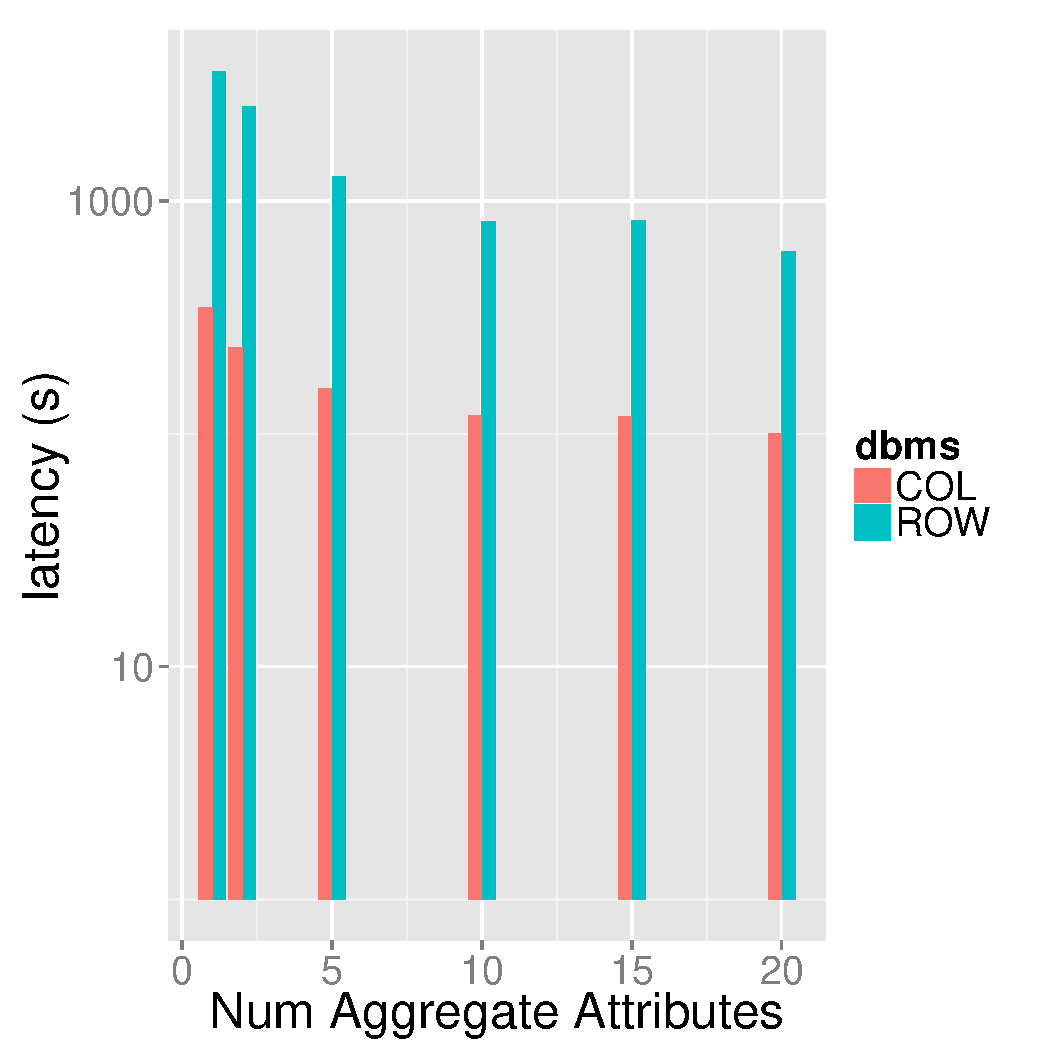
\includegraphics[width=6cm] {Images/multi_agg.pdf}}
% \caption{Latency vs. number of aggregates}
% \label{fig:multi_agg}
% \end{figure} 

\stitle{Combining Multiple Group-bys:} 
{\em \underline{Summary:} Combining multiple view queries with a single group-by attribute into a single query will multiple
grouping improves performance by 2.5X in row stores.}
We now study the effect of combining multiple queries each with a single group-by into one query.
Unlike the multiple aggregates optimization, the impact of combining group-bys
is unclear due to larger memory requirements as well as post-processing cost.
To verify our hypothesis that the ideal grouping must be one that keeps memory utilization
under a threshold, we ran an experiment with datasets SYN*-10 and SYN*-100 where
we varied the number of group-by attributes in \SeeDB-generated SQL queries ($n_{gb}$) 
between 1 and 10.
Since each attribute in SYN*-10 has 10 distinct values and that in SYN*-100
has 100, a query with $n_{gb}=p$ would require memory proportional to $\max(10^p,
num\_rows)$ for SYN*-10 and proportional to $\max(100^p, num\_rows)$ for SYN*-100.
The results of the experiment are shown in Figure \ref{fig:multi_gb_same}.
As the number of group-by attributes increases from 1 to 10, the latency of ROW (blue) decreases initially.
However, once the space budget (proxied by the number of distinct groups) exceeds 10000, latency increases significantly. \mpv{rewrite}
We see a similar trend for COL, but with a space budget of 100.\footnote{The different space
budgets can be explained based on the different internal parameteres and implementations of
the two systems.}
This empirically verified relation between memory usage and latency supports the use of 
our bin-packing optimization.

% We see that for the row-store, latency does improve (and then gets worse) as the
% number of group by attributes increases.  
% The best latency is obtained for 2 group by attributs in SYN3-100 and 4 attributes in SYN3-10.  
% This suggests that it is the number of distinct groups that matters most, since these 
% minima occur at 10,000 distinct groups in both cases (shown on \ref{fig:multi_gb_same} as the 
% two ``10000'' labels on the ROW lines).
% Beyond 5 attributes, the performance degrades drastically.  
%  For the column-store, we see a
% relatively small improvement in latency for 2 groups on SYN3-10, with 1 group being best for
% SYN3-100.  Here again it appears that the total number of groups (100 in the case of the column store) determines
% the overall optimal performance.
% After $10^5$ groups, the performance also becomes much worse for COL.

% In Section~\ref{sec:dbms_optimizations}, we described
%  how the impact of this optimization was not
% clear since it increases the total number of groups significantly and therefore
% leads to higher costs of processing intermediate results.
% To evaluate this optimization, we use the SYN3-10 and SYN3-100 datasets.
% We chose these datasets over SYN1 and SYN2 since we wanted to control
% the number of distinct groups in every attribute and consequently the number of
% distinct groups in every combination of attributes.
% In SYN3-10 for example, all dimensions have 10 distinct values and each
% dimension is independently generated. 
% Therefore, the total number of distinct
% groups produced by a query with $p$ group-by attributes is $\max(10^p,
% num\_rows)$.
% SYN3-100 similarly has 100 distinct values per attribute and produces
% $\max(10^p, num\_rows)$ groups for $p$ attributes.
% Our goal in these experiments is to determine if (a) combining multiple
% group-by attributes improved performance, and (b) whether it was the number of
% group-by attributes or the number of distinct groups produced by a query that
% predicted performance.

% We ran \SeeDB\ on SYN3-10 and SYN3-100, and varied the number of
% group-by attributes in view queries ($n_{gb}$) between 1 and 10.


% These results show that 1) combining group by attributes can improve performance, up to a point, and 2) the optimal
% number of attributes is determined by the total number of distinct groups that will result.  Different systems have a different
% number of optimal groups, and this number is somewhat implementation dependent.  The performance degradation with
% large numbers groups likely result from cache misses or other (non)-locality effects
% as the memory required for the grouping grows, or as the system switches to external algorithms for these
% operations.

% \begin{figure}[h]
% \centering
% \begin{subfigure}{0.49\linewidth}
% \centering
% {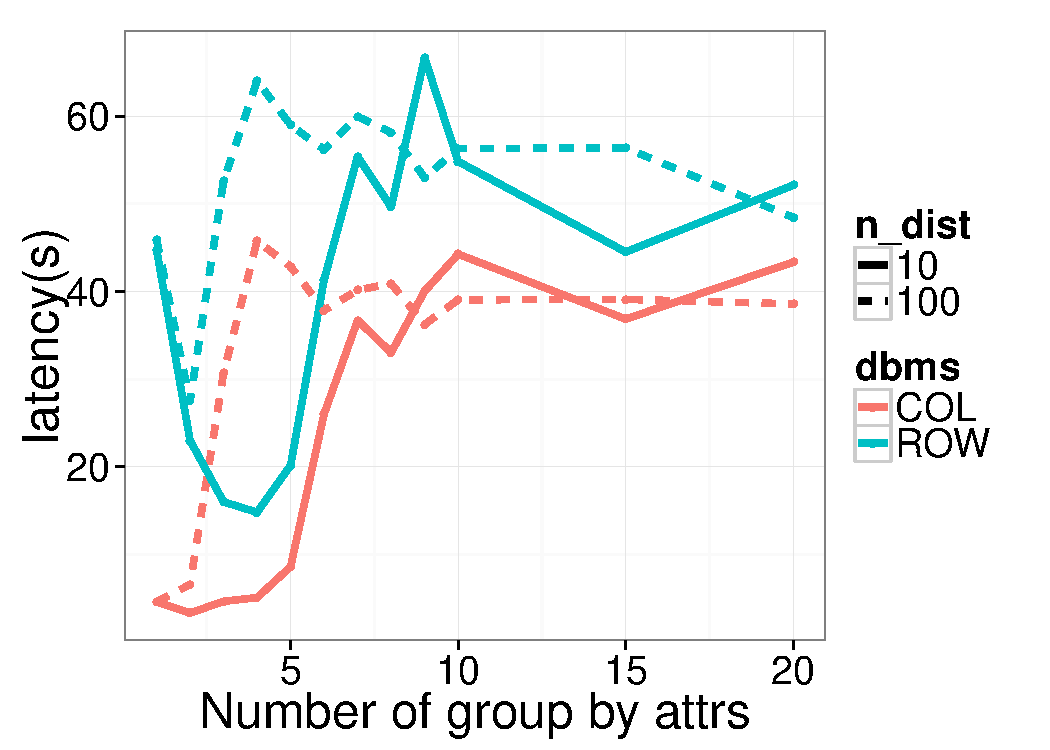
\includegraphics[width=4.2cm] {Images/multi_gb_same.pdf}}
% \caption{Latency vs. Num of Groups}
% \label{fig:multi_gb_same}
% \end{subfigure}
% \begin{subfigure}{0.49\linewidth}
% \centering
% {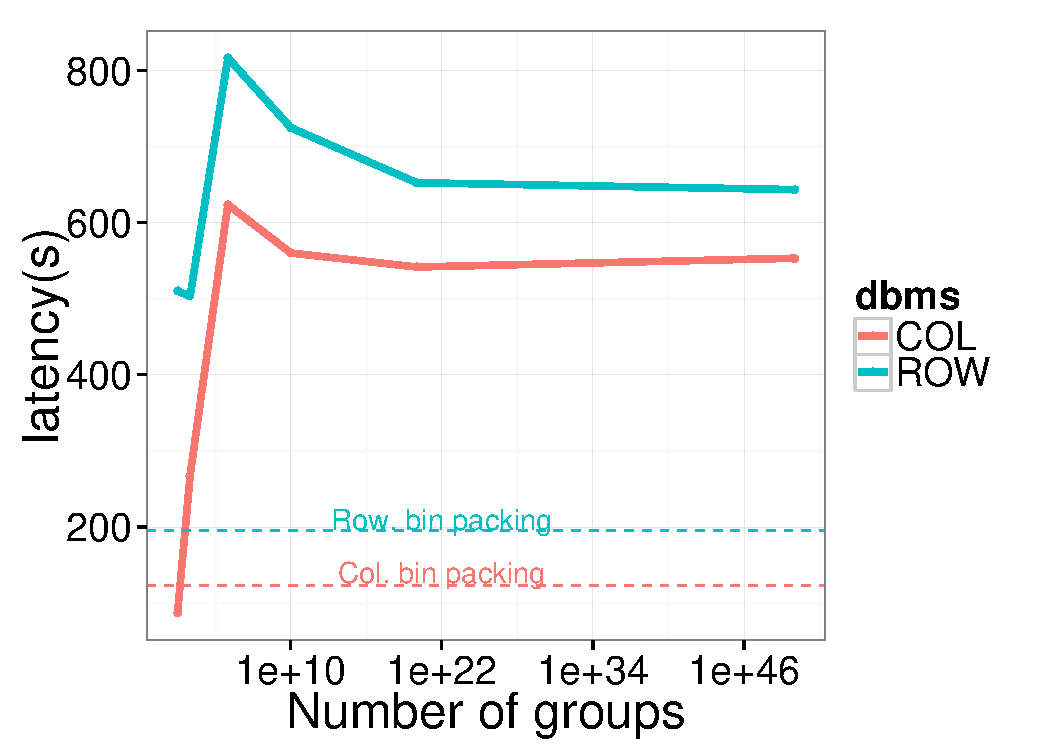
\includegraphics[width=4.2cm] {Images/multi_gb.pdf}}
% \caption{Latency vs. Num Dimensions}
% \label{fig:multi_gb_bp}
% \end{subfigure}
% \label{fig:multi_gb}
% \caption{Effect of combining multiple groups}
% \end{figure}

% We can guard against the above performance degradation by ensuring that the
% number of distinct groups never goes beyond a pre-configured upper limit.
% From Figure \ref{fig:multi_gb_same}, we see that this limit is approximately
% $10^4$ for the row-store and $10^2$ for the column store.

Next, we use the space constraint derived in the previous experiment
to perform optimal grouping via bin-packing (Section \ref{subsec:mult_gb}).
% With knowledge of this upper limit on the number of distinct groups, we can now
% apply our grouping technique based on bin packing (Section \ref{subsec:mult_gb}) to optimally
% group the dimension attributes.
% Bin-packing ensures that the number of distinct groups produced by any query is
% less than $10^4$ (for rows) or $10^2$ (for columns).
Figure \ref{fig:multi_gb_bp} shows the results of multi-attribute group-bys on SYN where
$n_{gb}$ was varied between 1 and 20 (solid lines).
Note that SYN contains attributes with variable number of distinct values (between 1 and 1000). 
Therefore, a query with
$n_{gb}$=3 can have memory utilization anywhere from 1 unit to $10^9$ units, thus breaking the
memory threshold.
Since the latency results in this experiment are greatly impacted by how attributes are grouped,
we randomize the grouping 20 times and report average latency.
The dotted lines show the latency obtained by performing optimal grouping via bin-packing.
We observe a significant, 2.5X improvement in ROW latency due to bin-packing.
This can be attributed to the fact that ROW's large threshold on space (10000) allows many queries
to be combined.
COL, on the other hand, shows a much less pronounced speedup. This is expected since its memory
threshold of 100 biases the optimal grouping to contain many single attribute groupings.
% To obtain these metrics, we randomly grouped attributes into groups of size $n_{gb}$ and ran
% the experiment 20 times to get average latency.
% We also show the performance of \SeeDB\ when we use bin-packing to optimally group the dimension
% attributes.
% As seen in the chart, grouping based on bin-packing is always superior to grouping based
% on the number of attributes $n_{gb}$. 
% In fact, for the row-store, bin-packing reduces latency by a factor of 2.5X. 
% Although benefit is less pronounced, it is also noticeable for column-stores.


% of bin packing when the number of groups is set to $10^2$ (columns) or $10^4$ (rows) (dotted lines).
% In the former strategy, we randomly group attributes into groups of size
% $n_{gb}$. 
% Since the latency for this strategy will depend on the particular grouping of
% attributes, we repeated this experiment 20 times and report the average latency.
% As we can see from the chart, bin-packing is always superior to grouping
% based on attribute number, given the optimal bin-size for a particular system.
% We see that for the row-store, bin-packing reduces latency by a factor of 2.5X. 
% Although benefit is less pronounced, it is still noticeable for column-stores.
 
%For other systems, we recommend users that they set the number of parallel
%queries to the maximum number of parallel queries that can be run in
%their DBMS without performance degradation.
%If this number is not easily available, a simple experiment as shown in Figure
%\ref{fig:parallelism} can help approximate the right amount of parallelism. \\

% \noindent {\it Combining Target and Comparison Views}:
% The last optimization we evaluate is that of combining the target and comparison
% views and running a single SQL query per view as opposed to two.
% We expected this optimization to roughly halve the latency since each query
% takes one table scan instead of two.\\

\begin{figure}[h]
	\centering
	\begin{subfigure}{0.48\linewidth}
		\centering
		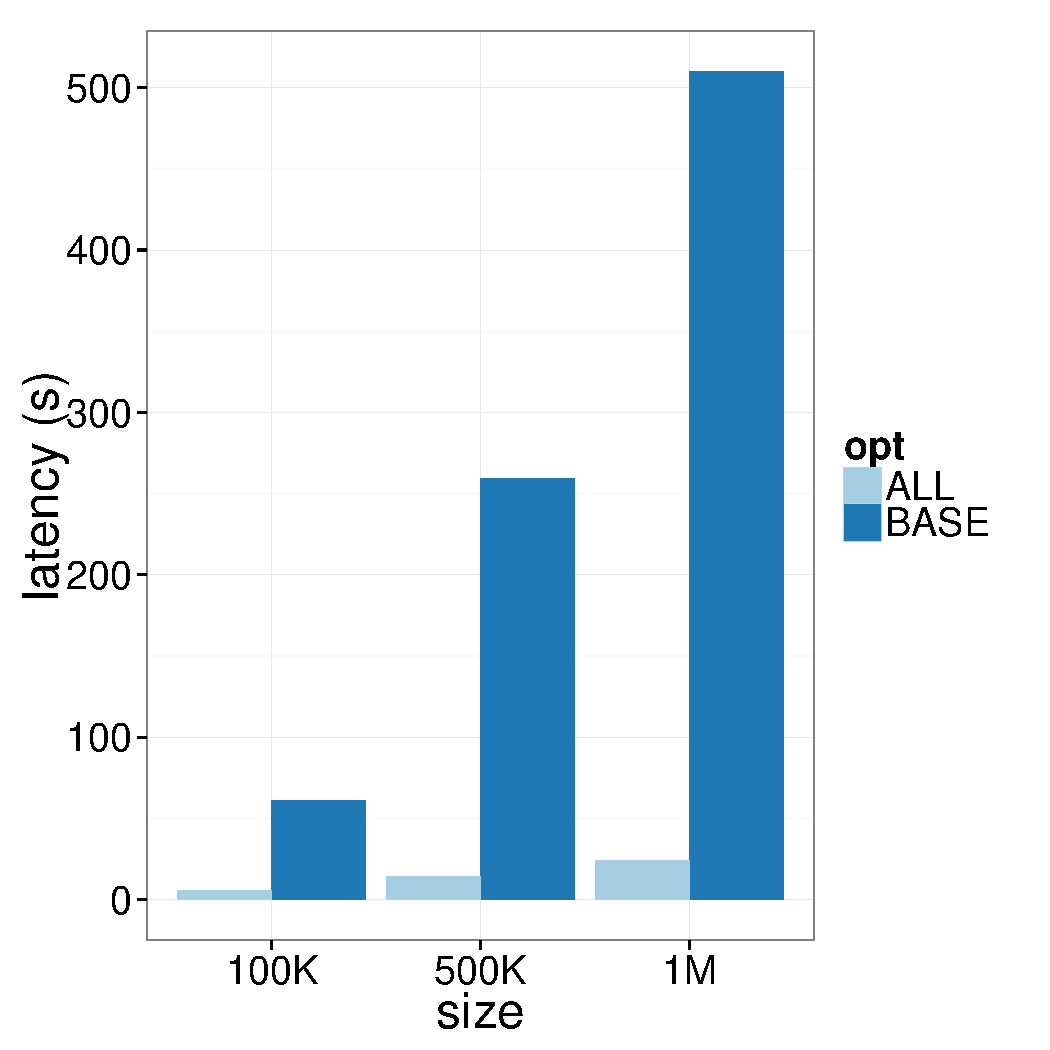
\includegraphics[width=4.4cm] {Images/row_all_none_by_size.pdf}
		\caption{Row store latencies by size}
		\label{fig:row_all_none_size}
	\end{subfigure}
	% \begin{subfigure}{0.24\linewidth}
	% 	\centering
	% 	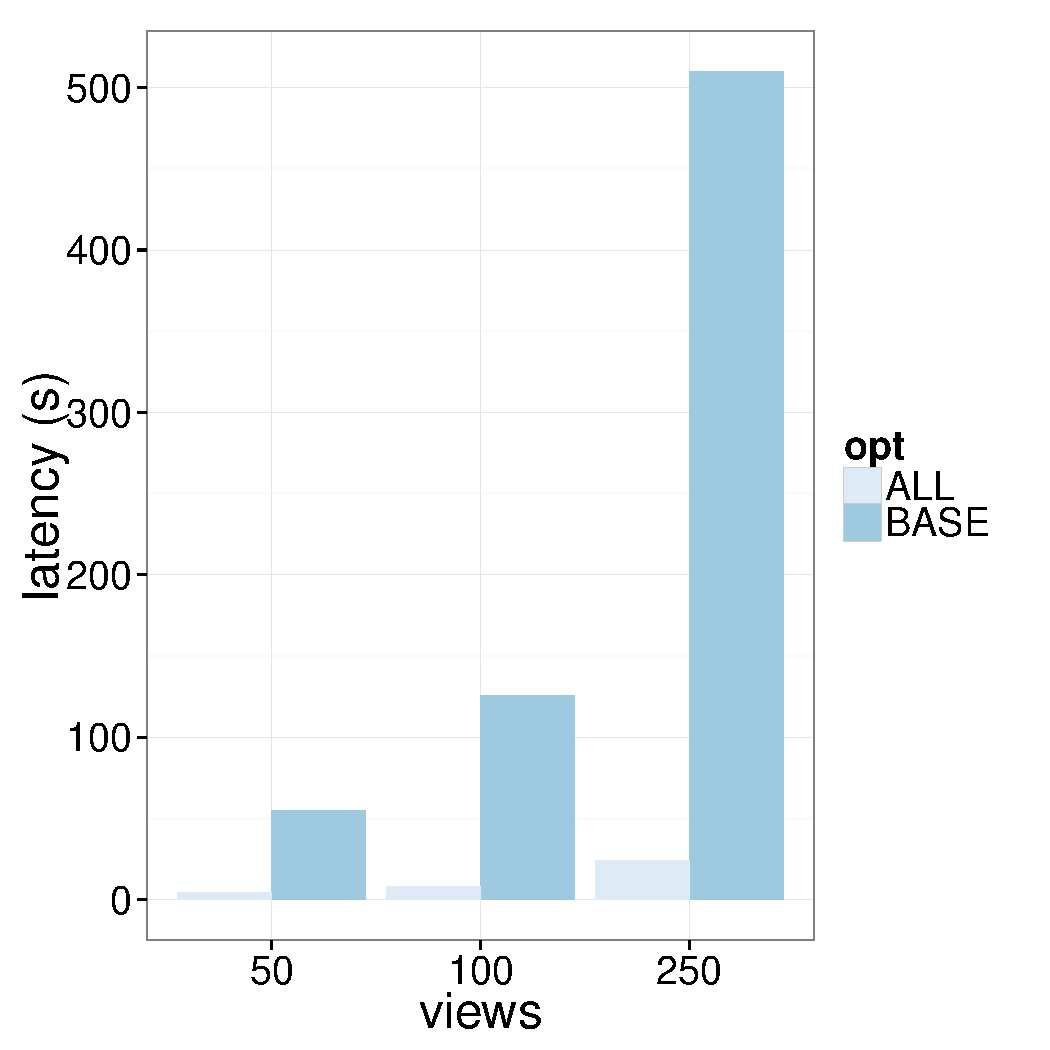
\includegraphics[width=4.6cm] {Images/row_all_none_by_views.pdf}
	% 	\caption{Row store latencies by views}
	% 	\label{fig:row_all_none_views}
	% \end{subfigure}
	% \begin{subfigure}{0.24\linewidth}
	% 	\centering
	% 	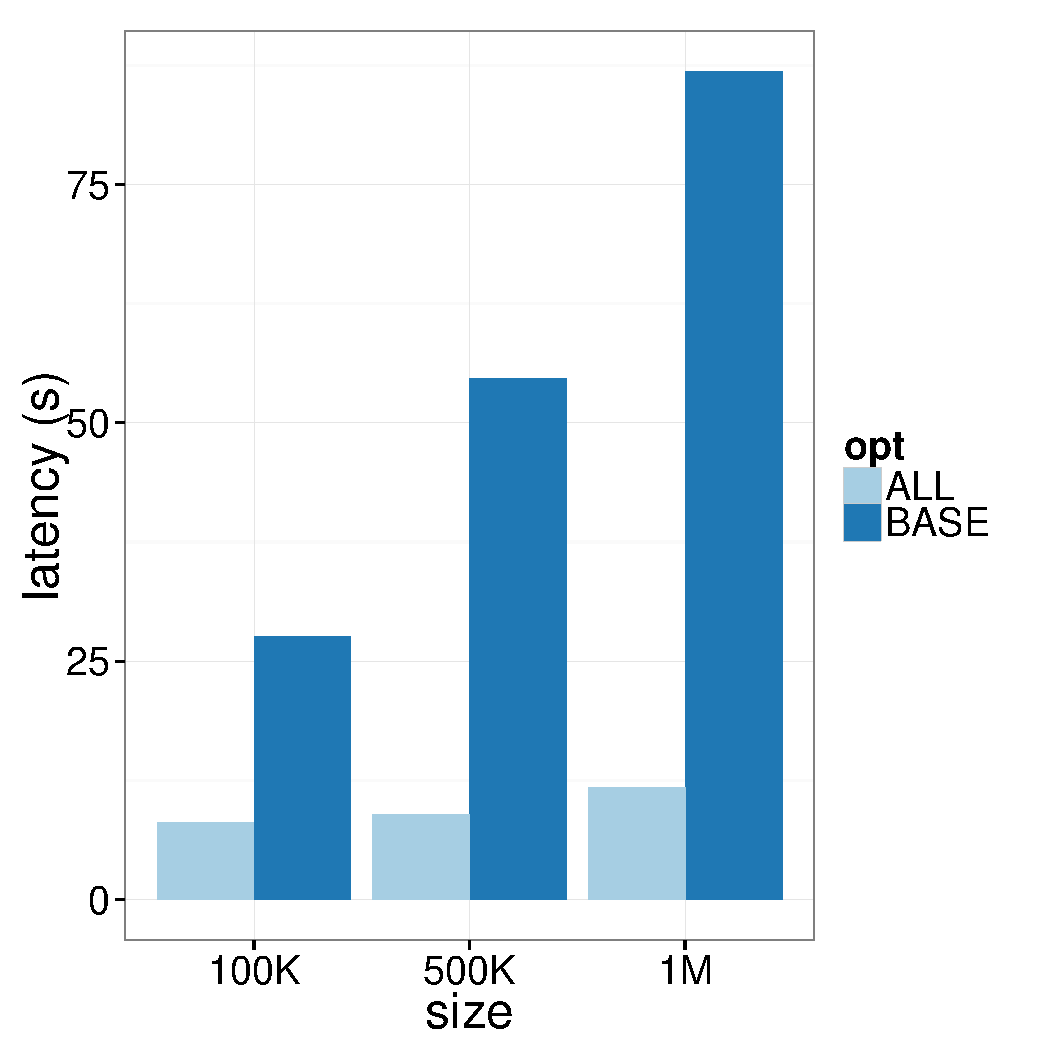
\includegraphics[width=4.6cm] {Images/col_all_none_by_size.pdf}
	% 	\caption{Column store latencies by size}
	% 	\label{fig:col_all_none_size}
	% \end{subfigure}
	\begin{subfigure}{0.48\linewidth}
		\centering
		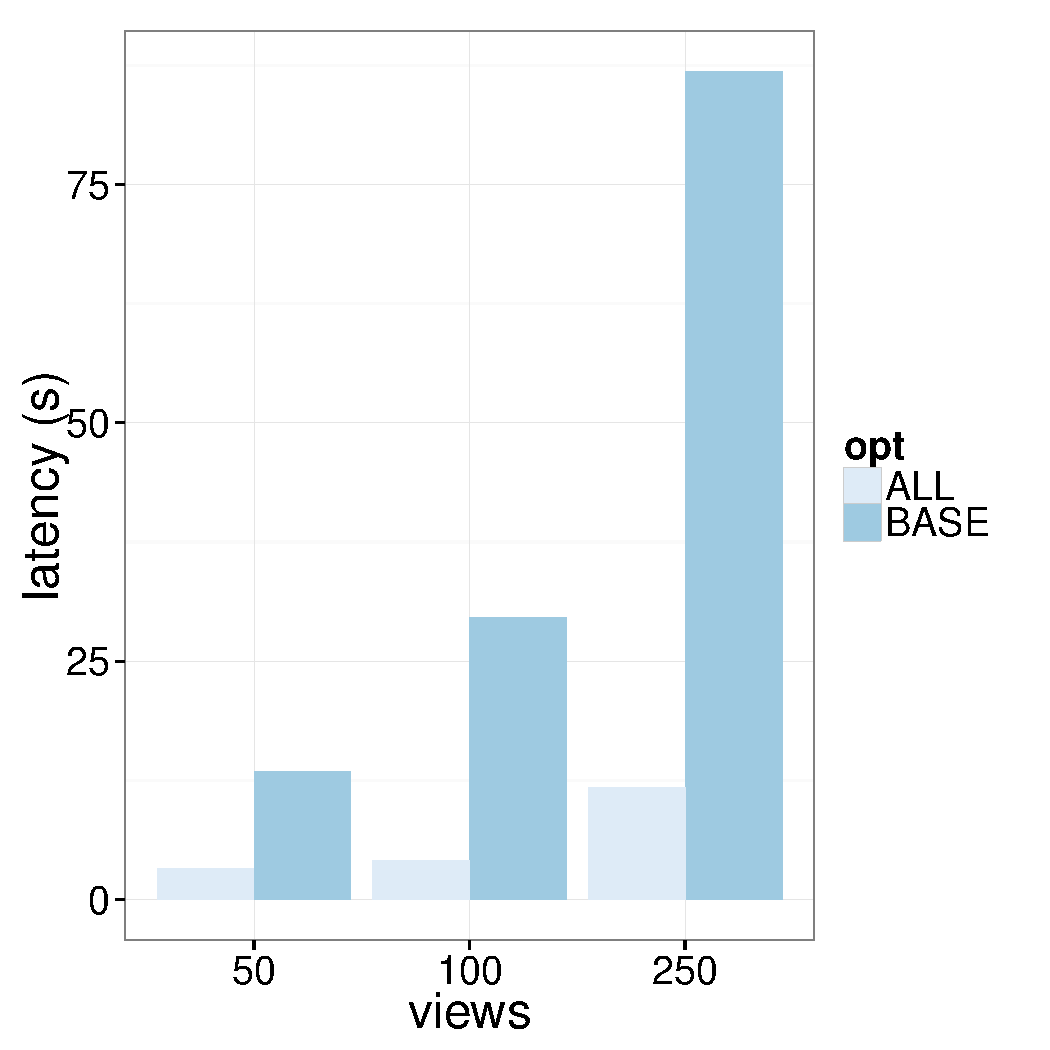
\includegraphics[width=4.4cm] {Images/col_all_none_by_views.pdf}
		\caption{Column store latencies by views}
		\label{fig:col_all_none_views}
	\end{subfigure}
	\vspace{-10pt}
	\caption{Effect of All Optimizations}
	\label{fig:all_opt}
	\vspace{-15pt}
\end{figure}


\stitle{All Optimizations:} 
{\em \underline{Summary:} Applying all of our optimizations together
leads to a speedup of up to 20X for row stores, and 8X for column stores;
column stores are still much faster than row stores.}
Based on the optimal parameters identified from the previous experiments, we combined 
our optimizations to obtain the best performance. 
% Now that we have explored the proposed optimizations in detail, we pick the optimal
% parameters discovered above and combine our optimizations to get the maximum
% performance gain. 
For the row store, we applied all the above optimizations with $n_{agg}$ set to
the total number of measure attributes, maximum number of group-bys set to $10^4$ and
parallelism set to $16$.
For the column store, we set $n_{agg}$ and number of parallel queries similarly
but did not apply the group-by optimization. 
Figure~\ref{fig:all_opt} shows the latency of \SeeDB\ on SYN when all
optimizations have been applied.
We see that our optimizations lead to a speed up of 20X for ROW 
(Figures~\ref{fig:all_opt}a) and a speedup of 8X in COL (Figures~\ref{fig:all_opt}b).
Furthermore, we notice that our optimizations are most effective for datasets with 
large sizes and many views.
% , with proportionally larger speedups as these numbers grow.

\stitle{Resource Utilization:}
Finally, we examine the resource utilization for the DBMS-backed engine.
With the DBMS-backed execution engine, each \SeeDB query translates into 50+ optimized SQL queries.
We call this 50X increase in queries as {\it query bloat}. 
Each SQL query scans the same data and stores individual state such as iterators, counters, buffers etc.
In addition, we find that although parallel queries share buffer pool pages, running a large number of view queries in
parallel can lead to thrashing due to timing issues.
As a result, we find the DBMS-backed engine has large overheads of memory, CPU and query state due to the query bloat.

In summary, the above set of experiments shows that the application of well-designed optimizations
and parallelism can reduce \SeeDB\ latency by 8-20X depending on the DBMS.
We notice, however, that in spite of aggressive optimizations, the latencies of DBMS-backed
\SeeDB are between 10-20s.
Such latencies are unacceptable in any interactive system.
Moreover, we observe that query bloat associated with each \SeeDB invocation unnecessarily consumes DBMS resources.
In an environment where the DBMS serves multiple users with more than just visualization
software, this approach is clearly wasteful. 
As a result, we see need for a solution that can provide much lower latencies 
and have a smaller resource footprint.
In the next section, we evaluate the performance of our custom execution engine that promises these advantages.
%!TEX root=document.tex

\subsection{Pruning Optimizations}
\label{sec:custom_execution_engine_expts}
In Section \ref{sec:in_memory_execution_engine}, we developed a set of strategies that enable \SeeDB to eliminate aggregate views with low utility early on and identify top-$k$ aggregate views rapidly.
Through the next set of experiments, we evaluate 
the impact of these optimizations.
% Specifically, our evaluation studies the impact of
% (a) our pruning strategies, 
% (b) utility distributions for the dataset, and (c) parameters of our heuristics
% on latency and accuracy.
% Specifically, in addition to latency (i.e. time required for \SeeDB to produce recommendations),
% we evaluate whether the views chosen by \SeeDB actually have the highest utilities.

\stitle{Metrics:}
We evaluate performance of pruning optimizations along two dimensions, {\em latency} and
quality of results.
We measure the quality of results in two ways: 
(1) {\em accuracy}: if $\{\mathcal{V}_T\}$
is the set of aggregate views with the highest utility and $\{\mathcal{V}_S\}$ is the set of aggregate views returned by
\SeeDB, the accuracy of \SeeDB is defined as $\frac{1}{\{|\mathcal{V}_T\}|} \times 
|\{\mathcal{V}_T\} \cap \{\mathcal{V}_S\}|$, i.e. the
fraction of true positives in the aggregate views returned by \SeeDB. (2) {\em utility distance}: since multiple
aggregate views can have similar utility values, we use utility distance as a measure of how {\it far} \SeeDB 
results are from the true top-$k$ aggregate views. 
Formally, using notation from Section \ref{sec:problem_statement}, we define utility distance as the difference between the average utility of $\{\mathcal{V}_T\}$ 
and the average utility of $\{\mathcal{V}_S\}$, i.e., $\frac{1}{n}(\sum_{i}U(\mathcal{V}_{T,i}) - 
\sum_{i}U(\mathcal{V}_{S,i}))$.

\stitle{Techniques:}
In the following experiments, we evaluate four techniques for pruning low-utility views.
In addition to the two pruning strategies from Section~\ref{sec:sharing_opt}, 
namely the Hoeffding Confidence Intervals (CI) and the Multi-Armed Bandit (MAB),
we implement two baseline strategies.
First, the no pruning strategy processes the entire data and does not discard any views (NO\_PRU). 
It thus provides an upperbound on latency and accuracy, and lower bound on utility distance.
The other baseline strategy we evaluate is the random strategy (RANDOM) that returns a random 
set of $k$ aggregate views as the result.
This strategy gives a lowerbound on accuracy and upperbound on utility distance: for any 
technique to be useful, it must do significantly better than RANDOM.
Finally, note that latencies of any pruning strategy depend closely on the execution techniques 
used within phases. 
For instance, using the basic \SeeDB framework (Section \ref{sec:dbms_exec_engine}) within each phase
will produce much larger latencies than applying all the sharing-based optimizations.
%In addition, each phase is associated with a fixed amount of overhead that depends on the DBMS.
Therefore, in this section, we will focus only on relative 
improvements in latency, specifically, the percent improvement in latency compared to latency
achieved without pruning.
Absolute latency numbers are discussed in Section \ref{sec:expt_summary}.

%we present latencies in this section 

\stitle{Datasets:}
We evaluate our pruning strategies on the real-world datasets from Table \ref{tab:datasets}. 
We describe the results for BANK and DIAB in this section while AIR and AIR10 are discussed 
in Section \ref{sec:expt_summary}. 
\techreport{
Specifically, we make use of the BANK and DIAB datasets listed in Table
\ref{tab:datasets}. 
Both datasets
contain a mix of numerical and categorical attributes. 
The diabetes dataset~\cite{diab} contains records of hospital visits by diabetes patients. Records include demographics,
diagnoses, number of hospital days, and procedures performed. 
The bank dataset~\cite{bank} contains records of customers who applied for a loan, including demographic information about 
the customers, information about the bank's previous contact with the customer, and the ultimate loan decision.
}





% For the custom execution engine, on the other hand, we are concerned with both, {\em latency} 
% as well as {\em accuracy}, i.e., whether \SeeDB actually returns the top-$k$ views or not.

\techreport {
\stitle{Result Highlights:}
\begin{denselist}
\item Our pruning strategies
reduce \SeeDB latency from 20 seconds (without pruning in custom engine) to less than 2 seconds
to return the first view, representing a {\em 10X reduction in latency}.

\item Our latency improvements do not impact accuracy significantly;
the accuracy of our results is $> 80\%$ with an almost zero utility distance.
% the utility diof the returned views are close to the utilities
% of the actual top-$k$ views.

\item The distribution of (true) view utilities impacts accuracy of pruning strategies.
Particularly, accuracy is inversely proportional to $\Delta_k$ the difference in
utility between the $k$-th highest utility and the two neighboring utilities. 

% \item Our technique of making a single pass through the data along with pruning reduces the overall
% resource utilization of \SeeDB compared to the DBMS engine \mpv{quantify}.

% \item Our  indicates that pruning significantly improves \SeeDB performance.
% In addition, our requirement of only a single pass through the data reduces resource utilization.
% Most importantly, 

\item In all, the latency reduction of 10X (for top few views) -- 2X (overall) along with low
utility distance enables \SeeDB to return high-quality recommendations {\bf at interactive time scales}.
This makes the custom execution engine a better alternative to a DBMS-backed engine
in terms of latency, accuracy as well as resource utilitzation (more in Section \ref{sec:comp_of_engines}).
\end{denselist}
}

% In addition to {\em latency}, we measure {\em accuracy},
% the number of true top-$k$ views present among the top-$k$ returned by the algorithm.
% In some cases, we will also measure {\em utility distance}, i.e., the 
% difference between the mean utility of the returned top-$k$ views
% and actual top-$k$ views.
% Unlike accuracy, which is 0-1, {\em utility distance}
% allows us to assess the benefit of strategies that return views with very high 
% (but not top) utilities.


% that have gone into We believe that comparing such
% systems offers little value:
% on one hand, our custom implementation lacks features such as logging or
% concurrency control that can slow down more complete systems; on the other hand,
% it also lacks optimizations for exploiting multiple cores, compression,
% vectorization, and other optimizations that scan-optimized column-stores employ.
% Rather, our goal is to highlight the relative performance benefits that can be
% obtained by performing pruning and shared scans.

\begin{figure}[h]
	\centering
	\vspace*{-10pt}
	\begin{subfigure}{1\linewidth}
		\centering
		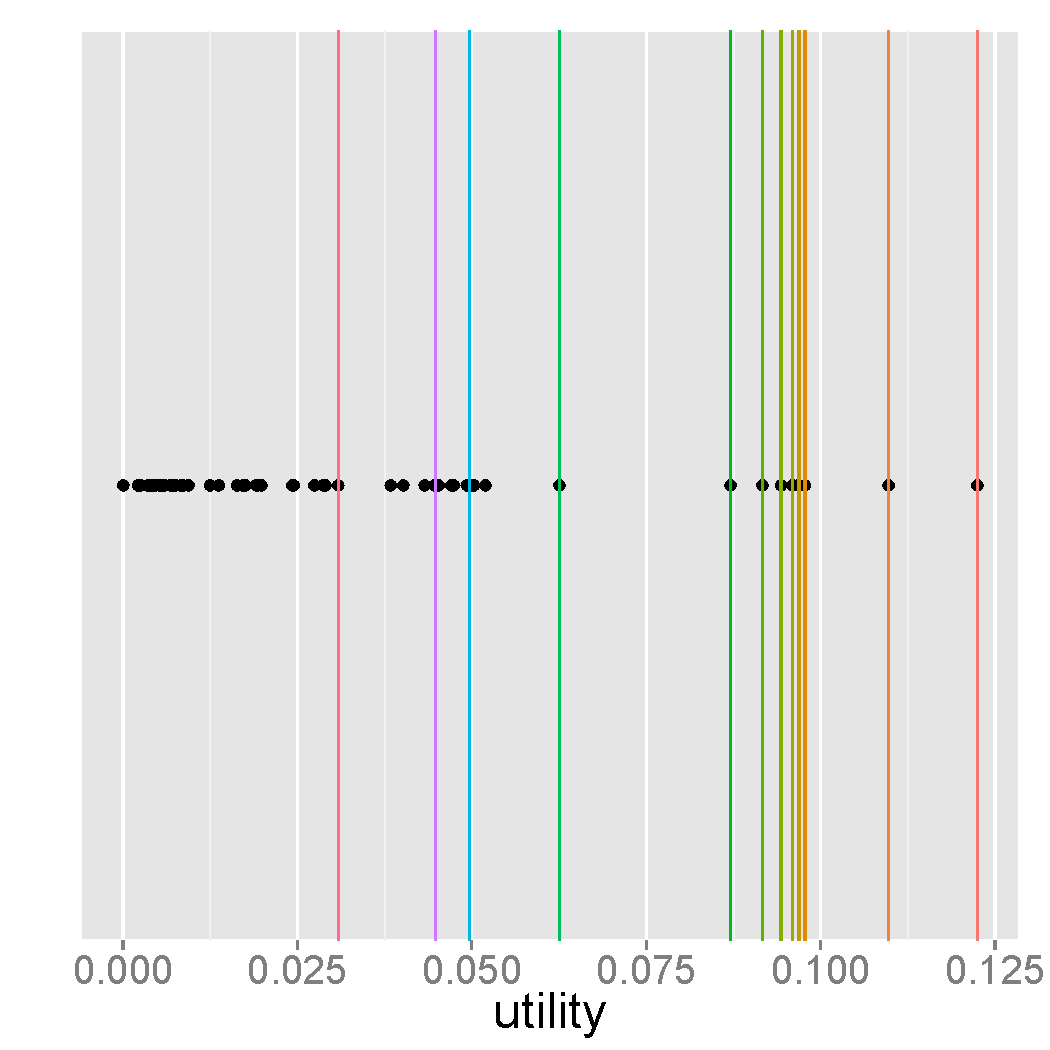
\includegraphics[width=6.5cm]
		{Images/bank_utility_distribution.pdf}
		\vspace{-5pt}
		\caption{Bank dataset: utility distribution}
		\label{fig:bank_utility_distribution}
	\end{subfigure}
	
	\begin{subfigure}{1\linewidth}
		\centering
		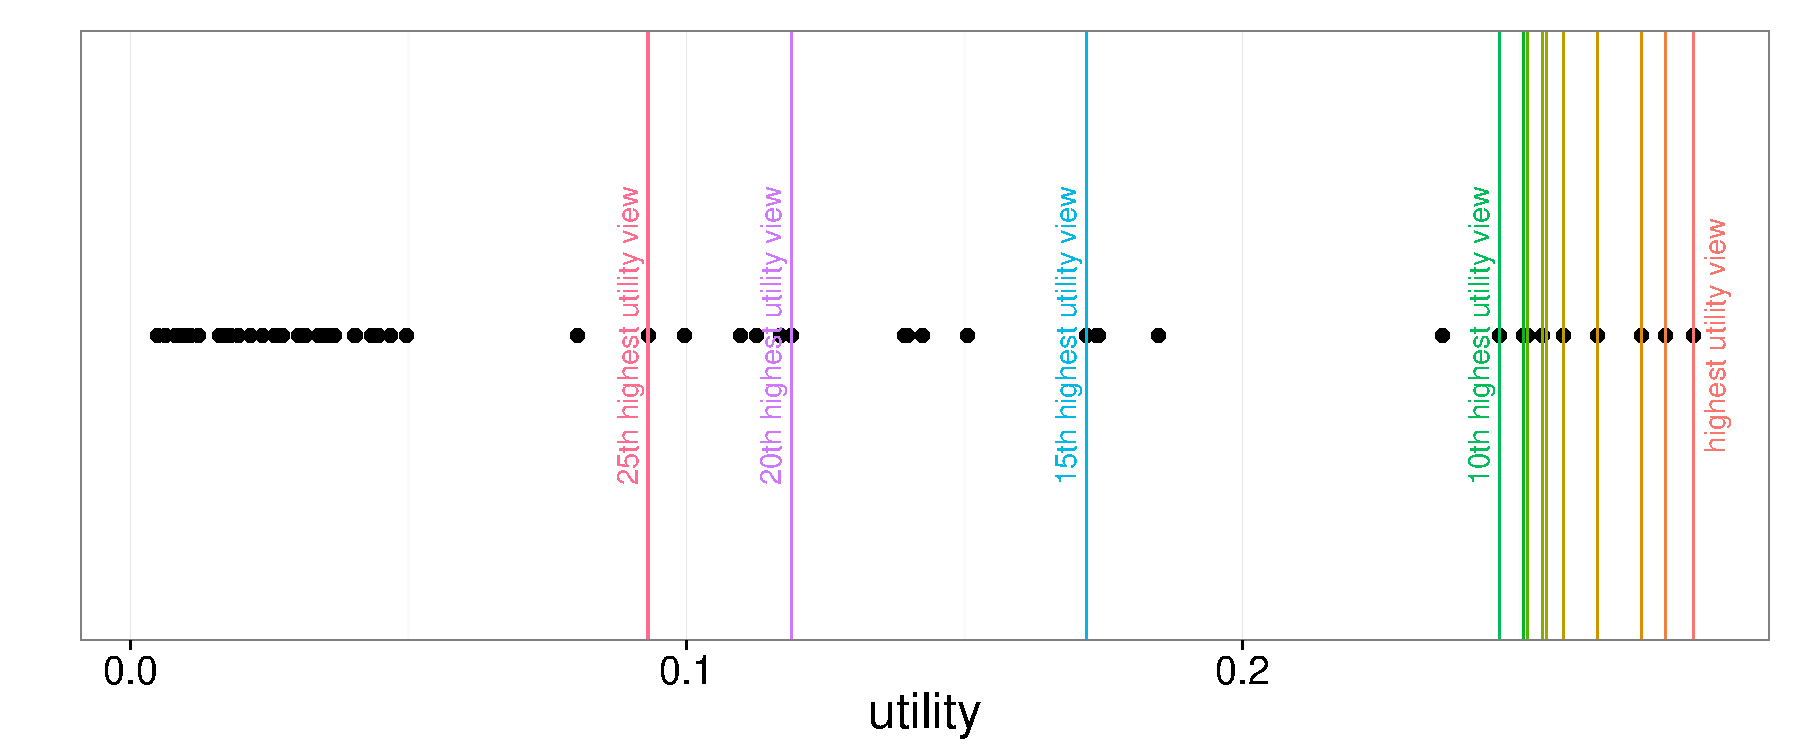
\includegraphics[width=6.5cm]
		{Images/diabetes_utility_distribution.pdf}
		\vspace{-5pt}
		\caption{Diabetes dataset: utility distribution}
		\label{fig:diabetes_utility_distribution}
	\end{subfigure}

\vspace{-10pt}
\label{fig:utility_distribution}
\caption{Distribution of Utilities}
\vspace{-15pt}
\end{figure}

In each of our experiments, we vary $k$ --- the number of aggregates views to select --- between
1 and 25 (a realistic upper limit on the number of aggregates views displayed on a screen)
and measure the latency, accuracy, and utility distance for each of our
strategies. 
Since the accuracy and utility distance of our techniques are influenced by the
ordering of data, we repeat each experiment 20
times and randomize data between runs. We report average
metrics over 20 runs.
% We note upfront that our goal is not to directly compare the latency of our custom
% execution engine to that of the DBMS-backed execution
% engine; comparisons between a commercial DBMS-backed system and a proof-of-concept
% system are futile.
% Instead, our goal is to evaluate the performance improvements that can be
% obtained by pruning \techreport{and sharing table scans }in our proof-of-concept 
% implementation.\footnote{We note however that for our experimental datasets, 
% the proof-of-concept prototype provides performance comparable to the DBMS-backed
% system.} We start with an evaluation of the quality of results produced by our custom execution
% engine.

% For example, the DBMS-backed engines (especially the column store) benefits from 
% many man-years of optimizations, including optimizations for scan-intensive workloads, 
% vectorization, compression, the ability to exploit multiple cores and so on.  







% \begin{compactenum}[(a)]
%  \item Hoeffding Confidence Intervals (CI): we use Hoeffding-Serfling
%  confidence intervals with overall $\delta = 0.05$; 
%  % \item 95\% Confidence Intervals (95\_CI): this pruning strategy uses normal 95\% confidence intervals; and 
% \item Multi-armed Bandit (MAB): this pruning strategy uses the multi-armed bandit algorithm.
% \item No Pruning (NO\_PRU): this strategy returns the top-$k$ views with highest utility,
% with no intermediate pruning (to study the impact of pruning on latency);
% \item Random (RANDOM): this strategy returns randomly selected $k$ views (to study the impact of pruning on accuracy).
% \end{compactenum}

\begin{figure*}[t]
	\centering
	\begin{subfigure}{0.33\linewidth}
		\centering
		{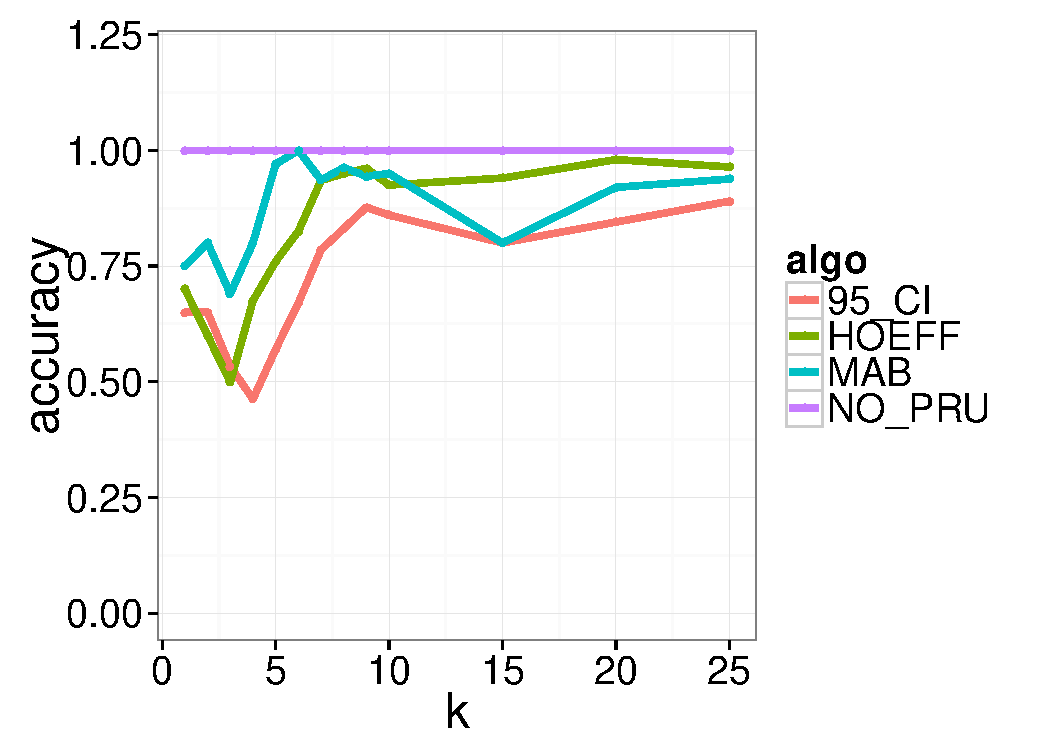
\includegraphics[width=6cm] {Images/in_memory_bank_accuracy.pdf}}
		\caption{Accuracy}
		\label{fig:bank_accuracy}
	\end{subfigure}
	\begin{subfigure}{0.33\linewidth}
		\centering
		{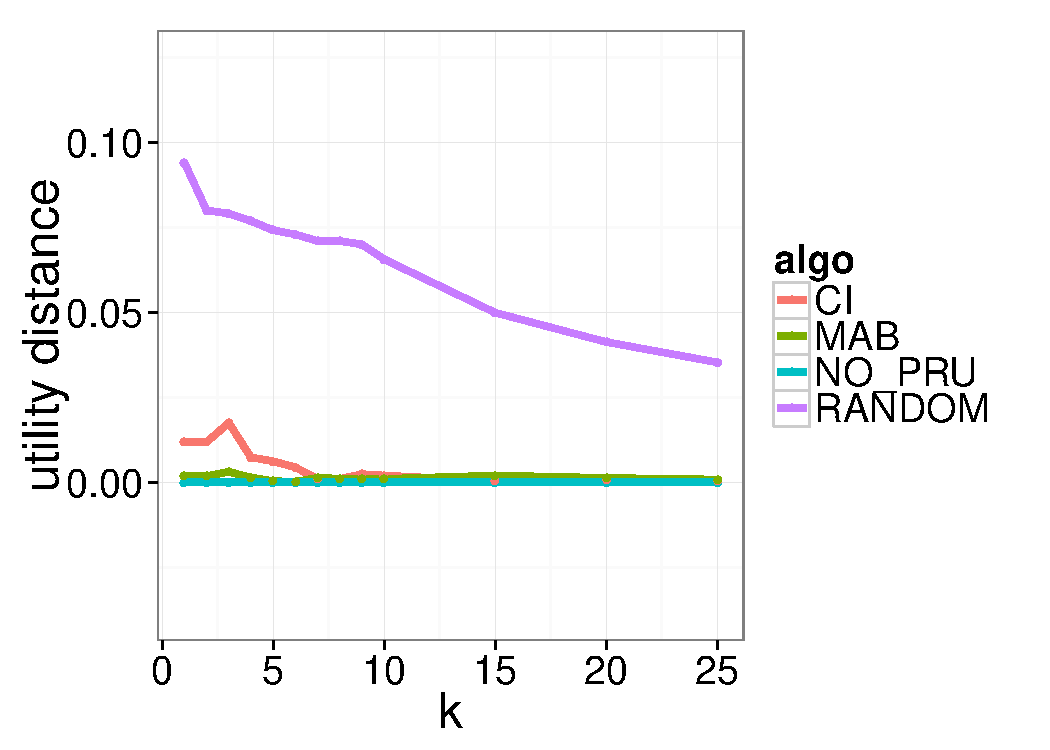
\includegraphics[width=6cm] {Images/in_memory_bank_utility_dist.pdf}}
		\caption{Utility Distance}
		\label{fig:bank_utility_dist}
	\end{subfigure}
	\begin{subfigure}{0.33\linewidth}
		\centering
		{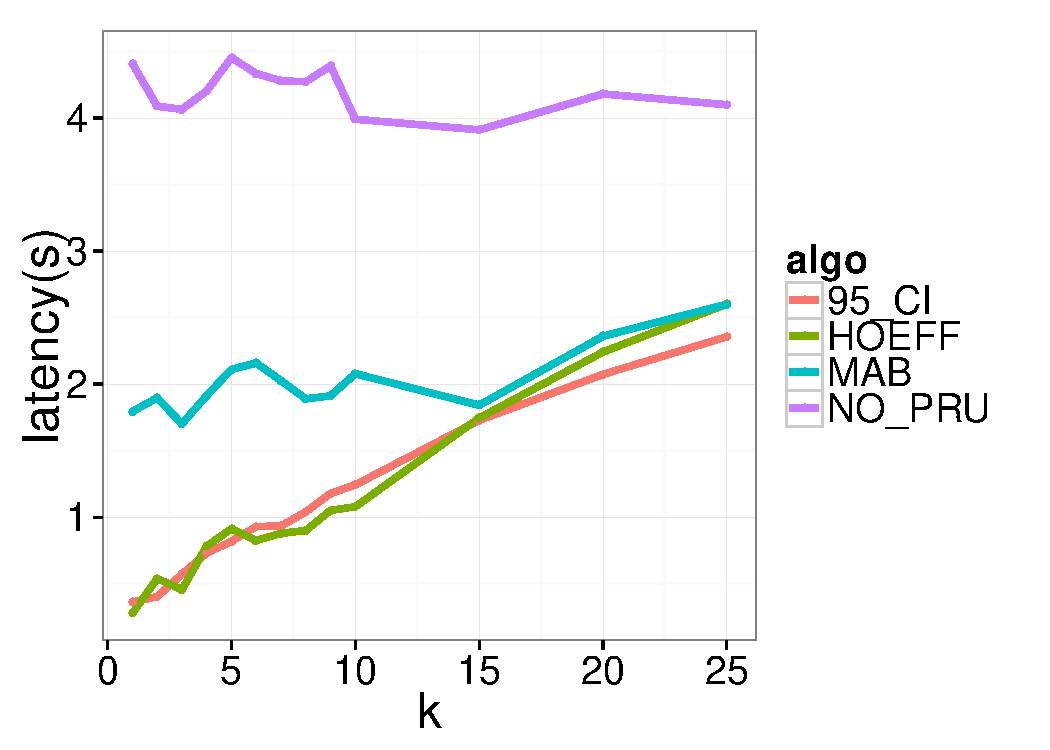
\includegraphics[width=6cm] {Images/in_memory_bank_latency.pdf}}
		\caption{Latency}
		\label{fig:bank_latency}
	\end{subfigure}
	\vspace{-10pt}
	\caption{Performance of strategies for Bank dataset}
	\label{fig:bank_perf}
	\vspace{-10pt}
\end{figure*}

\begin{figure*}[t]
	\centering
	\begin{subfigure}{0.33\linewidth}
		\centering
		{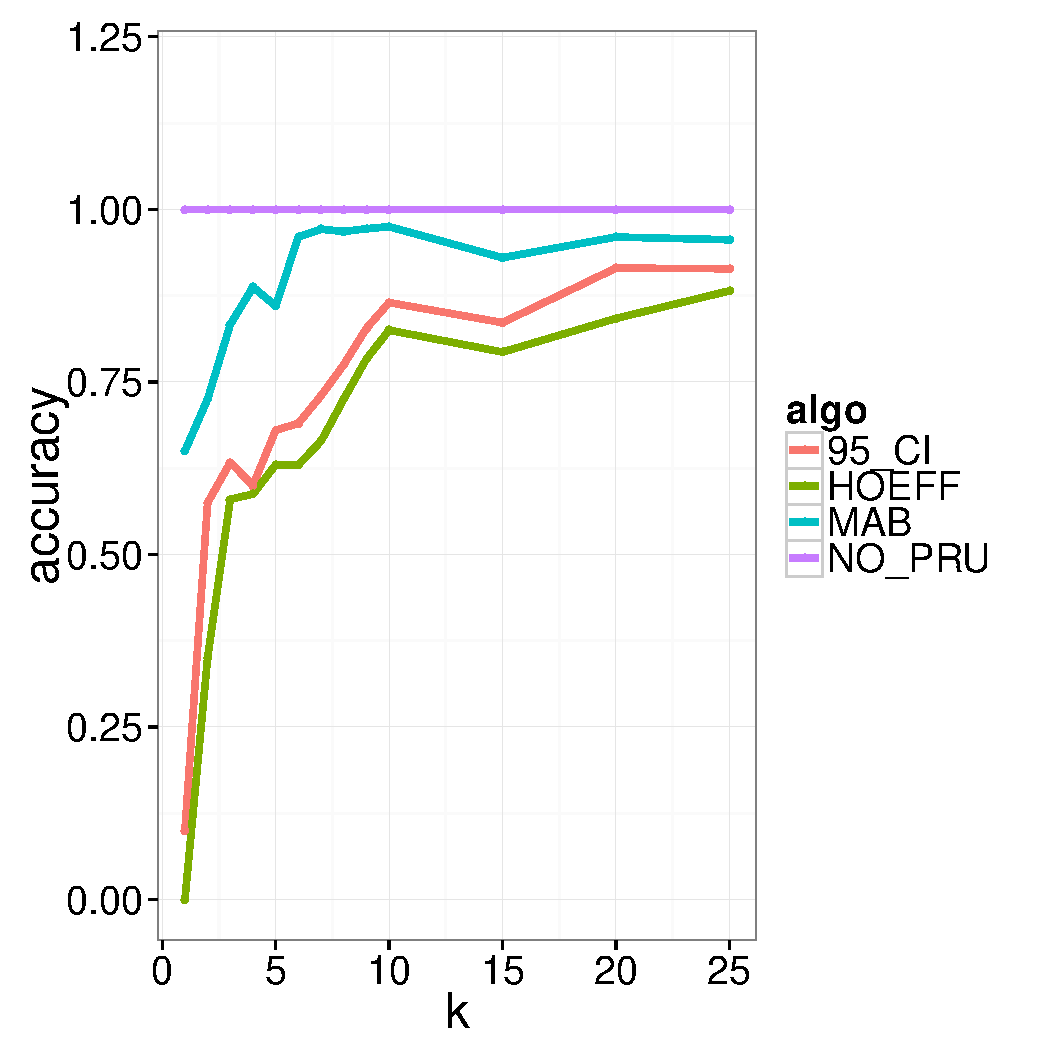
\includegraphics[width=6cm] {Images/in_memory_dia_accuracy.pdf}}
		\caption{Accuracy}
		\label{fig:dia_accuracy}
	\end{subfigure}
	\begin{subfigure}{0.33\linewidth}
		\centering
		{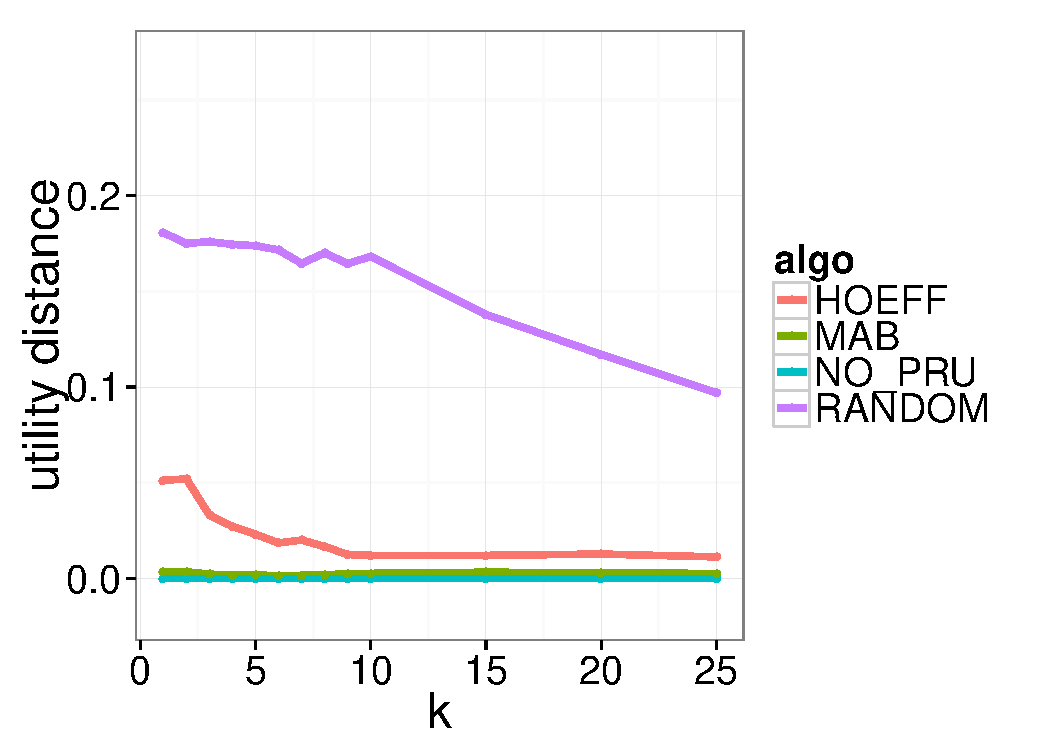
\includegraphics[width=6cm] {Images/in_memory_dia_utility_dist.pdf}}
		\caption{Utility Distance}
		\label{fig:dia_utility_dist}
	\end{subfigure}
	\begin{subfigure}{0.33\linewidth}
		\centering
		{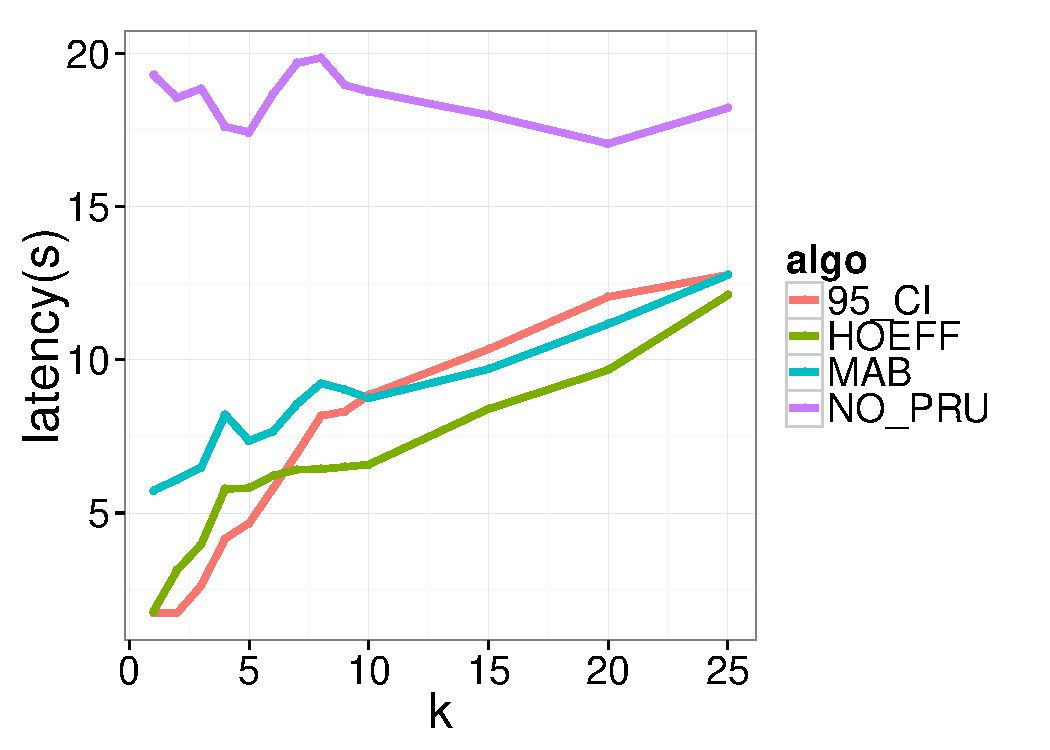
\includegraphics[width=6cm] {Images/in_memory_dia_latency.pdf}}
		\caption{Latency}
		\label{fig:diabetes_latency}
	\end{subfigure}
	\vspace{-10pt}
	\caption{Performance of strategies for Diabetes dataset}
	\label{fig:diabetes_perf}
	\vspace{-10pt}
\end{figure*}

 % \stitle{Utility Distributions and Quality of Results}:
 
 
 % Specifically, if a large number of views around the (true) top-$k$ boundary have similar utilities,
 % then our pruning strategies may choose views incorrectly at this boundary.
 % This results in lower accuracy.
 % On the other hand, since these views have utility similar to the true top-$k$ views, the
 % resulting utility distance is almost zero.
 %since utilities that are close together have very similar running
%estimates of utility and hence are difficult to tease apart and prune.
 % For each of the test datasets, we first review the utility distributions and then
 % analyze the performance of our pruning strategies given the utility distribution.

\stitle{Accuracy and Utility Distance:}
{\em \underline{Summary:} The MAB and CI strategy both produce results with 
accuracy $>$75\% and near-zero utility distance for a variety of $k$ values.
MAB does slightly better than CI when utlity values are closely spaced.
However, in general, smaller $\Delta_k$ values lead to lower accuracy, but this is offset by
lower utility distance that is a consequence of the smaller $\Delta_k$s. 
}

\noindent Since our pruning optimizations use utility estimates to prune aggregate views, 
 the accuracy of pruning depends on how accurately
 our estimates can capture the relative order of utilities.
 Aggregate views with utilities that are spread apart can be pruned accurately while
 those with similar utilities can lead to pruning inaccuracies.
 % have similar utility estimates and can lead to an incorrect ordering of views.
 The difference between utility values is particularly relevant at the top-$k$
 boundary.
 Reusing notation from the MAB technique, if $V_1 \ldots V_n$ is the list of aggregate views 
 ordered by decreasing utility, then the accuracy of pruning is inversely proportional to 
 the difference between the $k$-th highest utility and the $k+1$-st utility, 
 i.e., $\Delta_k = U(V_k) - U(V_{k+1})$.

%  \em \underline{Summary:} The MAB strategy dominates the CI
% strategy when it comes to both accuracy and utility distance,
% with accuracy $>$75\%  for $k = 1$ and even larger for larger
% values of $k$, and a near-zero utility distance. 
% Smaller $\Delta_k$ values lead to lower accuracy, but this is offset by
% lower utility distance.
%  }

\noindent {\it \underline {BANK dataset}}:
The distribution of utilities for all aggregate views of the bank dataset is
shown in Figure~\ref{fig:bank_utility_distribution}. 
In this chart, vertical lines denote the cutoffs for utilities of the top-$k$ views
where $k$=\{1,\ldots,10,15,20,25\}.
The highest utility for this dataset corresponds to the {\it right-most} line
in this chart while the 25-th highest utility corresponds to the {\it left-most}
line. 
We observe that the highest and second highest utility are spread well apart 
from the rest of them ($\Delta_k$=0.0125). 
The top 3rd--9th utilities are similar ($\Delta_k$<0.002) while the 10th highest 
utility is well separated from neighboring utilities ($\Delta_{10}$=0.0125).
The remaining aggregate views once again have similar utilities ($\Delta_k$<0.001).
We see the effect of of utility distribution in the performance of our pruning 
strategies.
Figure~\ref{fig:bank_accuracy} shows the {\it average} accuracy of our strategies over 20 runs.
We find that MAB consistently produces 75\% or better accuracy.
CI also produces 85\% or better accuracy for $k$$>$10.
For $k$=1 and 2, the accuracy is 75\% for both pruning strategies (due to large 
$\Delta_k$ values).
Between $k$=3\ldots9, the accuracy for all strategies suffers due to similar utility values 
($\Delta_k < 0.002$).
After $k$=10, the performance of all our strategies improves once again and tends to 100\% accuracy.
We note that NO\_PRU necessarily has perfect accuracy, while RANDOM has extremely poor accuracy (<0.25).
Figure~\ref{fig:bank_utility_dist} shows the utility distance for
all of our strategies.
% Next, we study the quality of our results in terms of utility distance. 
% Recall that utility distance measures how {\it far} our results are from the true top-$k$.
% Figure~\ref{fig:bank_utility_dist} shows the utility distance for
% all of our strategies for the bank dataset.
% The NO\_PRU technique necessarily has 0 utility distance since
% it performs no pruning.
We find that CI and MAB have zero or almost zero utility distance for all $k$, even where small $\Delta_k$s
lead to lower accuracy.
% RANDOM, on the other hand, has very high utility distance ($>$10X) compared to either of 
% CI and MAB.
This demonstrates the {\it paradox of pruning}: if aggregate views for a given $k$ have very small $\Delta_k$
values, the accuracy of our pruning techniques is lower; however, as a consequence of the small
$\Delta_k$ values, utility distance is also guaranteed to be small. 
Thus, in the worst case that \SeeDB picks a few aggregate views inaccurately, those views are guaranteed 
to have small utility distances.
% As with accuracy, the utility distance tends to zero with large $k$s.
% All our strategies produce views with 0 or almost 0 utility distance for most $k$. 
% Thus, even if \SeeDB picks a few incorrect views, there is effectively no difference in the 
% utilities of these views and the true top-$k$ views.
% So even when a top-$k$ strategy picks a few incorrect views, the selected views
% have utility very close to the real top-$k$ views, i.e., are views are
% of high quality.
% This implies that even if our top-$k$ views are
% approximate, they are of high quality.
% Another way to analyze mistakes in the top-$k$ views is by examining if the an
% incorrectly returned view for the top-$k$ views also appears in the top-$2k$,
% top-$3k$ or top-$4k$.
% Figure \ref{} shows the results for the banking dataset.
% We see that XXX,



% \begin{figure}[h]
% \centering
% \begin{subfigure}{0.49\linewidth}
% \centering
% {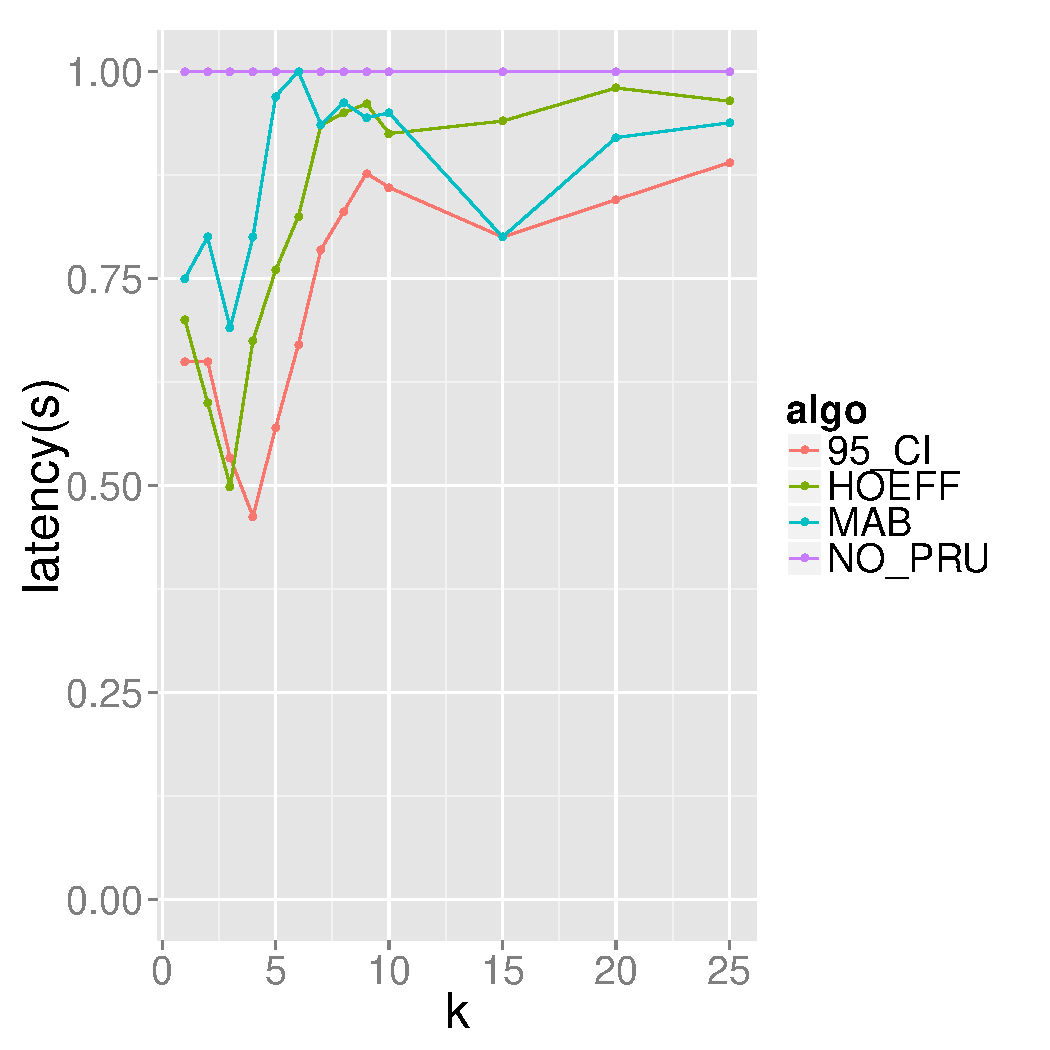
\includegraphics[width=4.2cm] {Images/bank_in_memory_accuracy.pdf}}
% \caption{Accuracy of strategy for bank dataset}
% \label{fig:bank_accuracy}
% \end{subfigure}
% \begin{subfigure}{0.49\linewidth}
% \centering
% {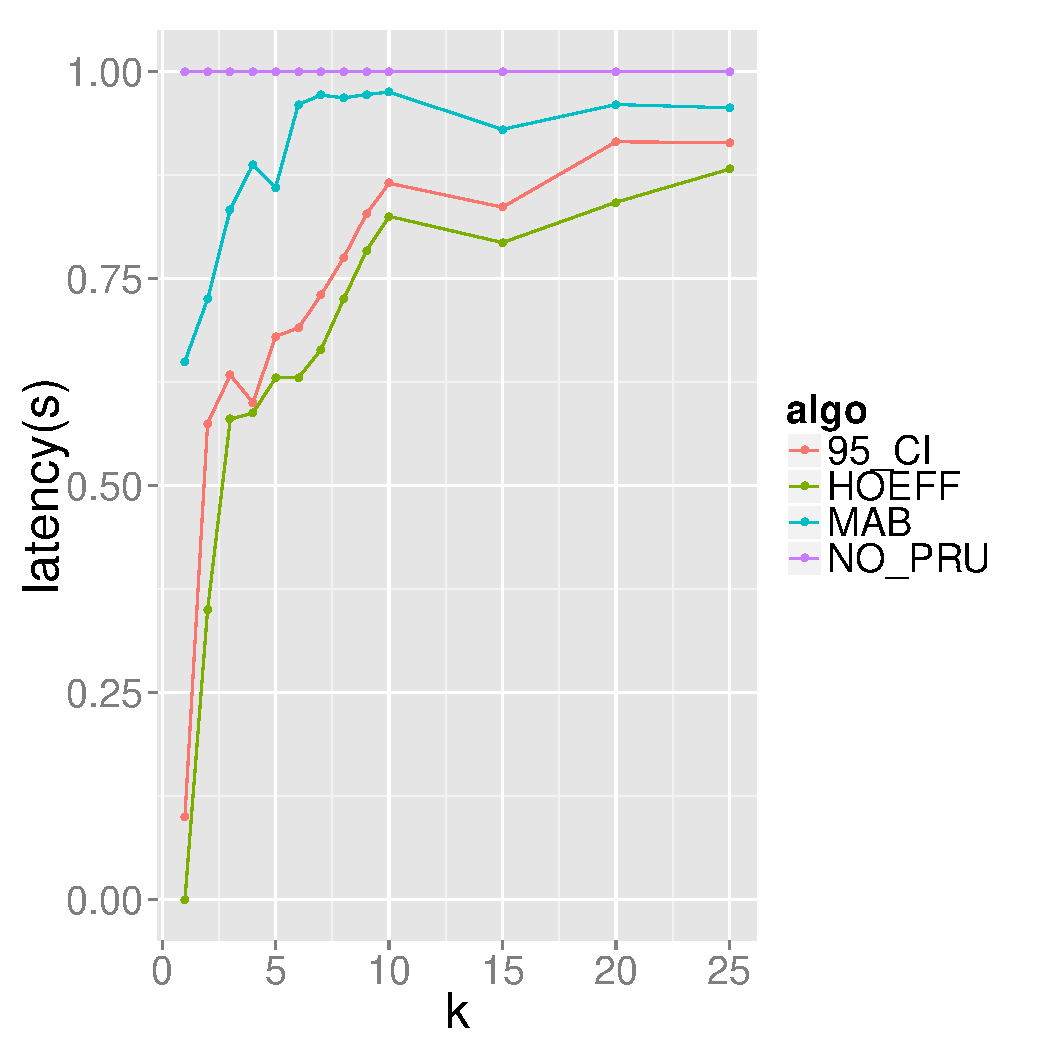
\includegraphics[width=4.2cm] {Images/dia_in_memory_accuracy.pdf}}
% \caption{Accuracy of strategies for diabetes dataset}
% \label{fig:dia_accuracy}
% \end{subfigure}
% \label{fig:accuracy}
% \caption{Accuracy of strategies}
% \end{figure}


% \begin{figure}[h]
% \centering
% \begin{subfigure}{0.49\linewidth}
% \centering
% {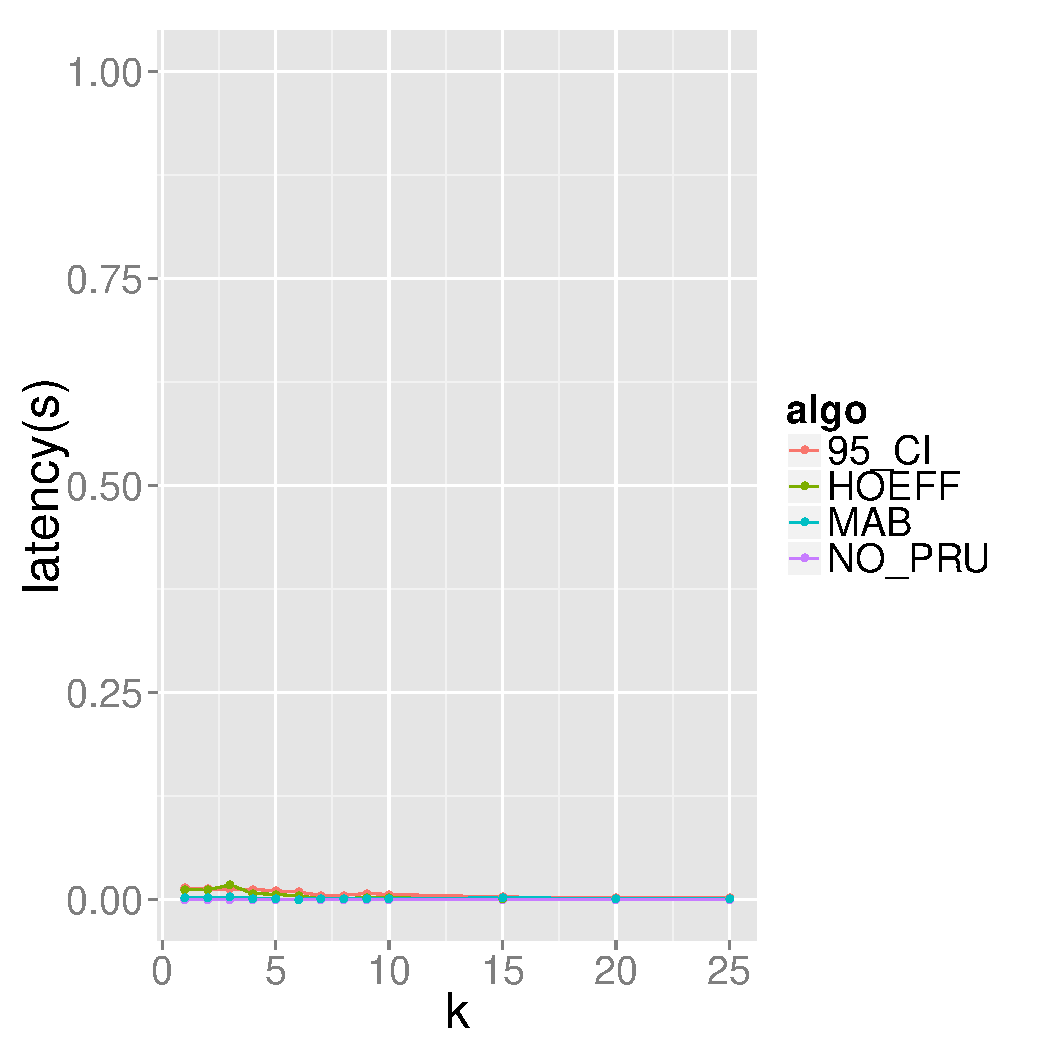
\includegraphics[width=4.2cm] {Images/bank_in_memory_utility_dist.pdf}}
% \caption{Utility Distance of strategy for bank dataset}
% \label{fig:bank_utility_dist}
% \end{subfigure}
% \begin{subfigure}{0.49\linewidth}
% \centering
% {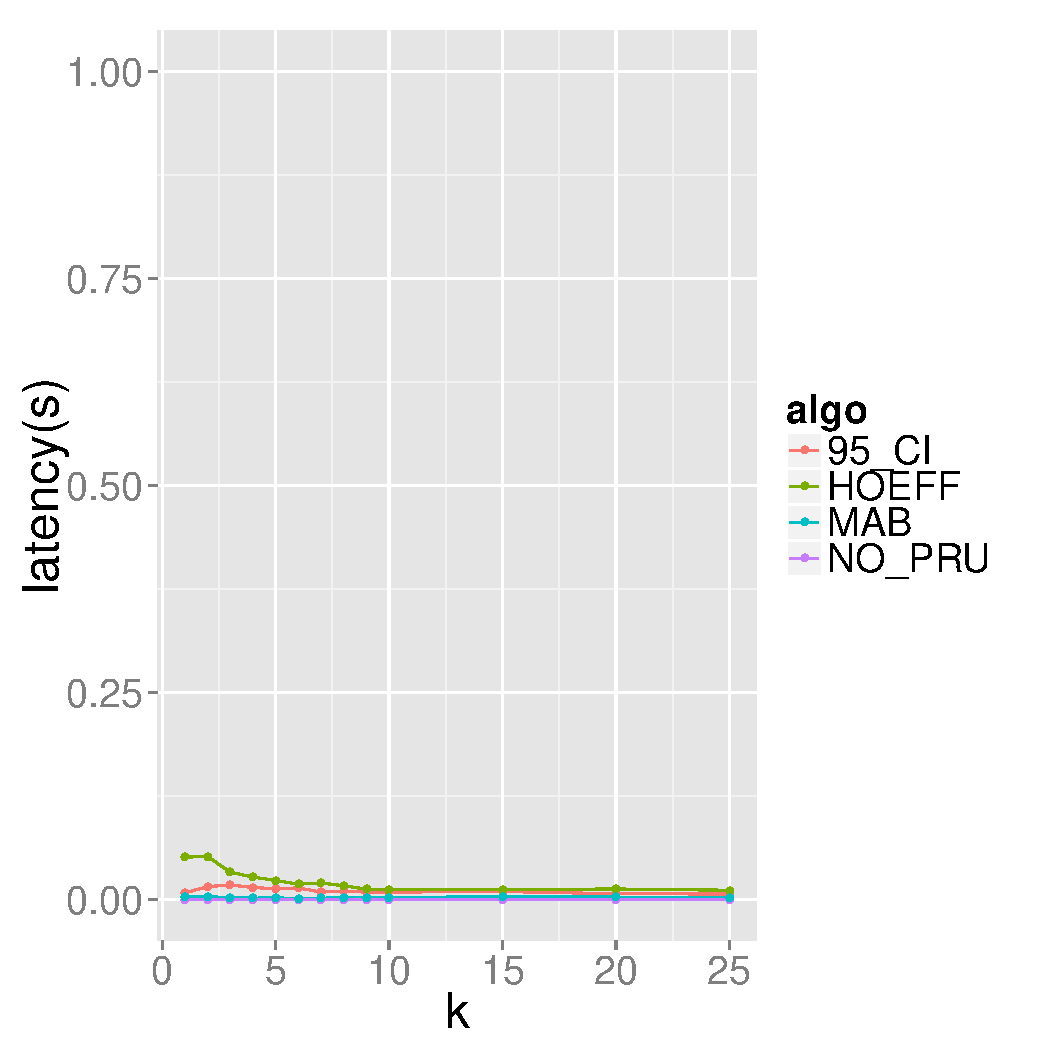
\includegraphics[width=4.2cm] {Images/dia_in_memory_utility_dist.pdf}}
% \caption{Utility Distance of strategies for diabetes dataset}
% \label{fig:dia_utility_dist}
% \end{subfigure}
% \label{fig:accuracy}
% \caption{Utility Distance for strategies}
% \end{figure}

% \begin{figure}[h]
% \centering
% {\includegraphics[trim = 0mm 50mm 0mm 50mm, clip, width=6cm]
% {Images/bank_utility_distribution.pdf}}
% \caption{Bank dataset: utility distribution}
% \label{fig:bank_utility_distribution}
% \end{figure}
% \begin{figure}[h]
% \centering
% {\includegraphics[trim = 0mm 50mm 0mm 50mm, clip, width=6cm]
% {Images/diabetes_utility_distribution.pdf}}
% \caption{Diabetes dataset: utility distribution}
% \label{fig:diabetes_utility_distribution}
% \end{figure}
 
\noindent {\it \underline{DIAB dataset:}} 
Next, we briefly review results for the the diabetes dataset.
The distribution of true utilities for all aggregate views in this dataset are shown in
Figure~\ref{fig:diabetes_utility_distribution}.
We observe that utilities for the top 10 aggregate views are very closely clustered ($\Delta_k<$0.002) while
they are sparse for larger $k$s.
Therefore, we expect lower pruning accuracy for $k<10$ but high accuracy for
large $k$'s.
We see this behavior in Figure~\ref{fig:dia_accuracy} where the accuracy of
pruning is quite low ($<60\%$) for $k$=1 but improves consistently to $k$=10 
($>80\%$) and is $>80\%$ for larger $k$s.
% \item View corresponding to $k$=15 is well separated from its neighboring views, $\Delta_{16} >$ 0.025
% \item Views for $k$=20 and 25 are also surrounded by utilities with very 
% similar values ($\Delta_k < $0.001).
% \end{denselist}
% We notice the MAB performs consistently better than CI even when the utility
% values are very similar.
% While NO\_PRU has perfect accuracy, RANDOM performs poorly. \mpv{NEED DATA}
In Figure~\ref{fig:dia_utility_dist} we see that
utility distance is small for $k<10$ and then reduces to almost 0 for larger
$k$s.
Both CI and MAB produce 40X smaller utility distances compared to RANDOM.
% Thus, we observe that both our strategies CI and MAB produce high quality results 
% in terms of accuracy as well as utility distance. 
% While the quality depends on the distribution of utilities, particularly on the 
% $\Delta$s at the top-$k$ boundary.
For the most commonly used $k$ value, $k$=10, we find that our strategies obtain 
90\% or more accuracy.

% We also observe an important property of our strategies: the accuracy of both
% of our pruning strategies, MAB and CI, is comparable; MAB appears to
% perform better for small number of $k$s but all three produce similar results
% for $k>10$. (NO\_PRU is guaranteed to have perfect accuracy).
% This suggests that since all strategies perform similarly on accuracy, we can
% choose the strategy with the minimum latency.\\

% 95\_CI does the best among all our strategies for the whole range of $k$ values.
% MAB and HOEFF produce similar accuracy values with MAB being slightly better
% than HOEFF.
% There are a few reasons why 95\_CI performs better: the MAB strategy is tied to
% either accepting or discarding a view at the end of each phase; therefore, even
% if MAB is not very confidence in the action of accepting or discarding, it must
% reduce one view in each phase. HOEFF on the other hand is less accurate because
% XXX.
% All our strategies however seem to have low accuracy for $k<10$. 

\stitle{Latency:}
{\em \underline{Summary:} All strategies provide a reduction in latency of 50\% or more
relative to NO\_PRU. For smaller $k$, reductions can be even higher, closer to 90\%; this can be
especially useful when we want to identify and quickly display the first one or two top views.}
Figures~\ref{fig:bank_latency} and \ref{fig:diabetes_latency} show the latency
of our strategies for the banking and diabetes dataset.
First off, we observe that the use of either of CI or MAB produces a 50\% reduction in latency
throughout.
In fact, for CI, we obtain almost a 90\% reduction in latency for small $k$. 
MAB, on the other hand, has a consistent 50\% reduction in latency. 
As expected, as $k$ increases, latency also increases because we can prune fewer aggregate views.
% These reductions bring latency down from multiple tens of seconds to {\bf single digit latencies}, i.e.,
% \SeeDB can operate on interactive time scales.
% Since these latency numbers come from our prototype implementation, a well-tuned system could
% produce results in few seconds, i.e., {\it in interactive time scales}. 
% Clearly, we give up some accuracy when we obtain this reduction in latency, however, as demonstrated
% experimentally, our strategies consistently provide high utility views with low utility distance.op-$k$.
% This latency-accuracy tradeoff is particularly important in a real-time system where we want to quickly 
% provide recommendations for the analyst to browse.
We note that MAB has a worse performance compared to CI since MAB can only discard a 
{\it single} view during each phase; CI in contrast has no upperbound on the number of aggregate views that it
can discard.
Consequently, MAB must execute a larger number of phases compared to CI, making it less attractive
when latency is paramount (e.g. when querying large datasets).

\techreport{
\stitle{Resource Utilization:}
% \mpv{Not sure about this section. Someone needs to review}
% We contrast the resource utilization of our custom execution engine to the DBMS-backed engine. 
% Specifically:
Compared to the resource utilization in the DBMS-backed engine, our custom engine requires much fewer resources.
Specifically, since the custom engine makes a single pass through the data, the CPU utilization is expected to be lower compared to the repeated scans of the DBMS-backed engine.
Another consequence of the single scan is that there is
no thrashing introduced by multiple parallel scan queries.
Lastly, there is no {\it query bloat} associated with
the custom engine, saving overheads of per-query state such as iterators, buffers etc.
}
% means that the custom engine is expected to
% have lower CPU as compared to the multiple scans of data resulting from the DBMS-backed engine (assuming that the
% additional state maintenance is not significant).

% Each \SeeDB query translates to only a single query in the custom execution engine.
% The DBMS-backed engine, in contrast, issues $~$ 50 queries for each \SeeDB query. 
% Consequently, additional resources must be wasted by the DBMS in keeping state for each query such as 
% iterators, buffers etc.

\techreport{
\subsection{Comparison of Execution Engines}
\label{sec:comp_of_engines}

The previous sections discussed the performance of the DBMS-backed and Custom execution engines of \SeeDB.
We found that with a set of clever optimizations, we could reduce the latency of the DBMS-backed engine by
20X.
However, the resulting latency of few tens of seconds was too large for interactive visualization.
In addition, we found that the query bloat led to large memory footprint, repeated scans of data, and
higher resource utilization.
In contrast, the custom engine provided a means to perform a single scan of the data and identify top-$k$ views
with high accuracy. \mpv{numbers?}
Moreover, the custom engine produced latencies of a few seconds -- {\bf it enabled \SeeDB to respond at interactive
time scales}.
These performance results together indicate that the custom execution engine and its pruning strategies are a superior 
alternative to a DBMS-backed execution engine.
Since the goal of \SeeDB is to provide recommendations in real time, we can pay a small penalty in accuracy 
and instead provide almost instantaneous results.

Clearly, the ideal solution would be to integrate the custom execution engine functionality into a vanilla database.
This would enable the DBMS to use existing structures to efficiently scan a dataset while maintaining and pruning
views on the fly. 
The SQL GROUPING SETS\footnote{} functionality, i.e. multiple independent group-bys in a single query is a first step in this direction.
However, GROUPING SETS needs to be supplemented with much finer control and scalability to support \SeeDB-like  functionality.}

% In summary, the performance results of this section indicate that due to the lower latency, high accuracy,
% and overall lower resource utilization, the custom engine is a superior alternative to a DBMS-backed
% execution engine.
% It enables \SeeDB to make a single pass through the data, avoids unnecessary {\it query bloat} leading to
% lower resource utilization and lowers latency by upto 10X enabling \SeeDB to work in a real 
% interactive visualization system.

% so all of these strategies are promising alternatives to use 
% in a production system --- especially when we want to quickly identify and provide a few 
% views for the analyst to browse.
% If latency is paramount, then CI may be used,
% and if utility is paramount, then MAB may be used. \mpv {counter-intuitive}
% We observe that the latency of CI increases almost linearly
% with $k$. This trend arises because as $k$
% increases, we throw out fewer views and therefore perform more
% computation per record.
% This exact trend is not seen in MAB because MAB's view pruning is agnostic
% to the number of views that must be selected.

% \subsection{Combining Sharing \& Pruning}
% \label{sec:sharing_and_pruning}
% As discussed in the previous sections, sharing optimizations can provide performance gains upto 10X for COL and 40X for ROW while pruning optimizations can reduce latency by 2X -- 5X.
% In this section, we evaluate the performance gains that can be obtained by combining both types of optimizations. 
% In the ideal case, we expect the gains to be {\it multiplicative}, i.e., we would expect gains between 20X -- 200X.



% Figure \ref{fig:share_prune_col} shows the relative performance gains that can be obtained by applying various combinations of optimizations in the COL store. 
% As seen in figure, 

% The corresponding data for ROW stores was presented in Figure~\ref{fig:share_prune_row} above.
% We find that the combination of optimizations produce gains of upto 50X (COMB) -- 150X (COMB\_EARLY) for ROW, with pruning-based
% optimizations providing a 4X speedup over the sharing optimizations.


% We see similar results for ROW where pruning provides a similar 4X speedup.
% However, we make a few observations. First, pruning doesn't benefit small datasets (e.g. BANK, DIAB). In fact, due to the overhead of multiple phases (and the associated query costs), the combined optimization (COMB) does worse than SHARING alone. Since the SHARING latencies for small datasets are under a few seconds, we do not find the need to perform sharing.
% Second, as noted before, due to different data layout, COL stores have significantly lower latencies for the \SeeDB workload compared to ROW.
% However, the data layout for ROW benefits more from the sharing of scans and pruning since the cost of a table scan is much higher for ROW.
% T
% COL stores in general are a better fit for the \SeeDB workload.

% Compared to the performance of ROW stores in Figure \ref{}, we find that COL stores benefit less from optimizations.
% As before, this is because column stores can selectively load attributes that are relevant for the particular visualization. \mpv{verify}

% % We also find a few differences in the performance gains obtained by pruning in Section \ref{} () and those obtained by the combined optimizations ().

% The reasons for this difference are two-fold: (1) the simple pruning implementation described in Section \ref{} is based on shared scans and does not incur any overhead for each phase of the algorithm; in contrast, when we implement pruning in \SeeDB, each phase involves \SeeDB issuing a large number of queries to the DBMS and thus incuring overheads such as query dispatch, maintaining query state etc. (2) due to the specific implementations of ROW and COL stores, there is threshold on table size below which the time to scan tables is essentially the same.
% As a consequence of these two factors, we find that the combination of pruning and sharing degrades performance for small datasets (e.g. BANK, DIAB) due to phase overhead.
% The combination of optimizations is well suited to moderate and large datasets such as AIR and AIR10 and produces a CCC speedup.



% The next set of experiments vary the parameters for each strategy to study
% the accuracy vs. latency tradeoff.

% \begin{figure}[h]
% \centering
% \begin{subfigure}{0.49\linewidth}
% \centering
% {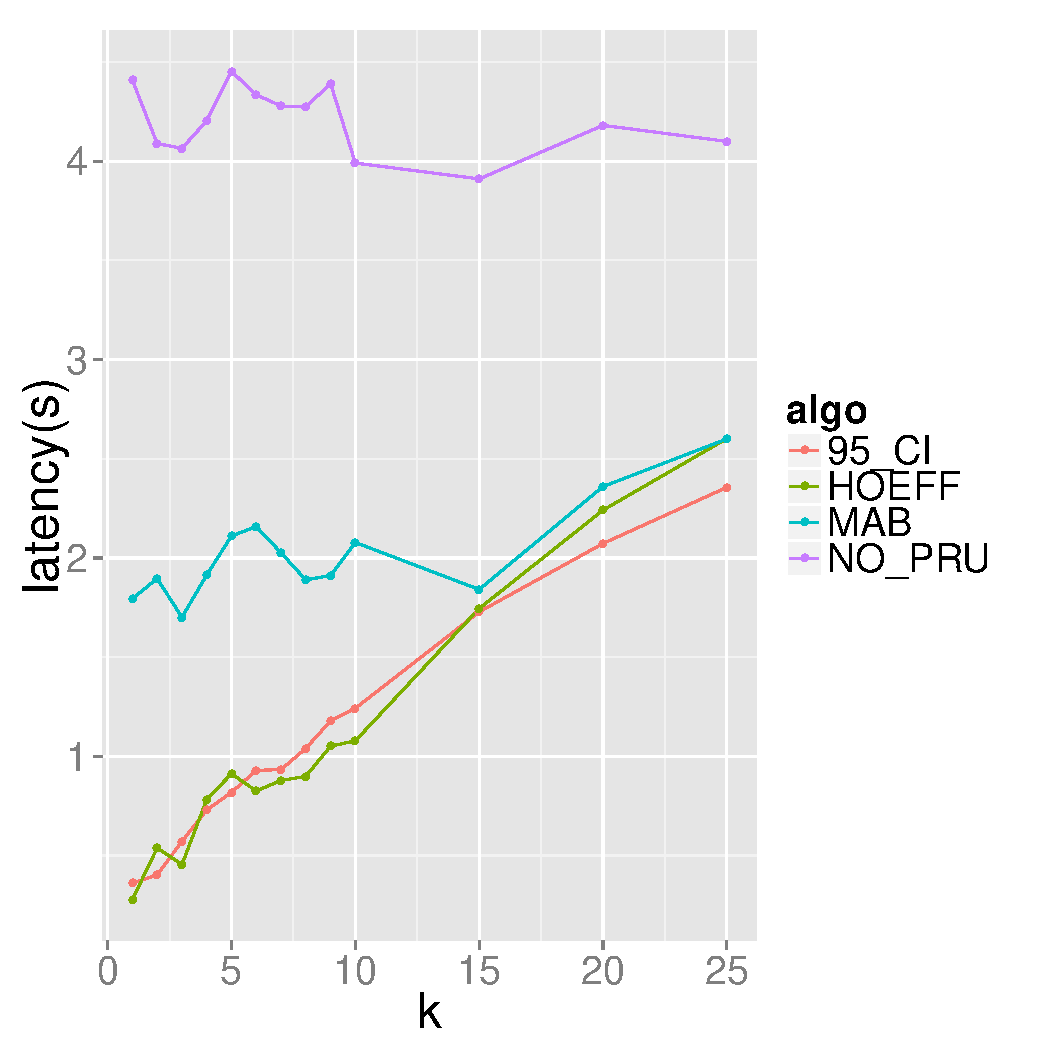
\includegraphics[width=4.2cm] {Images/bank_in_memory_latency.pdf}}
% \caption{Bank dataset: latency}
% \label{fig:bank_latency}
% \end{subfigure}
% \begin{subfigure}{0.49\linewidth}
% \centering
% {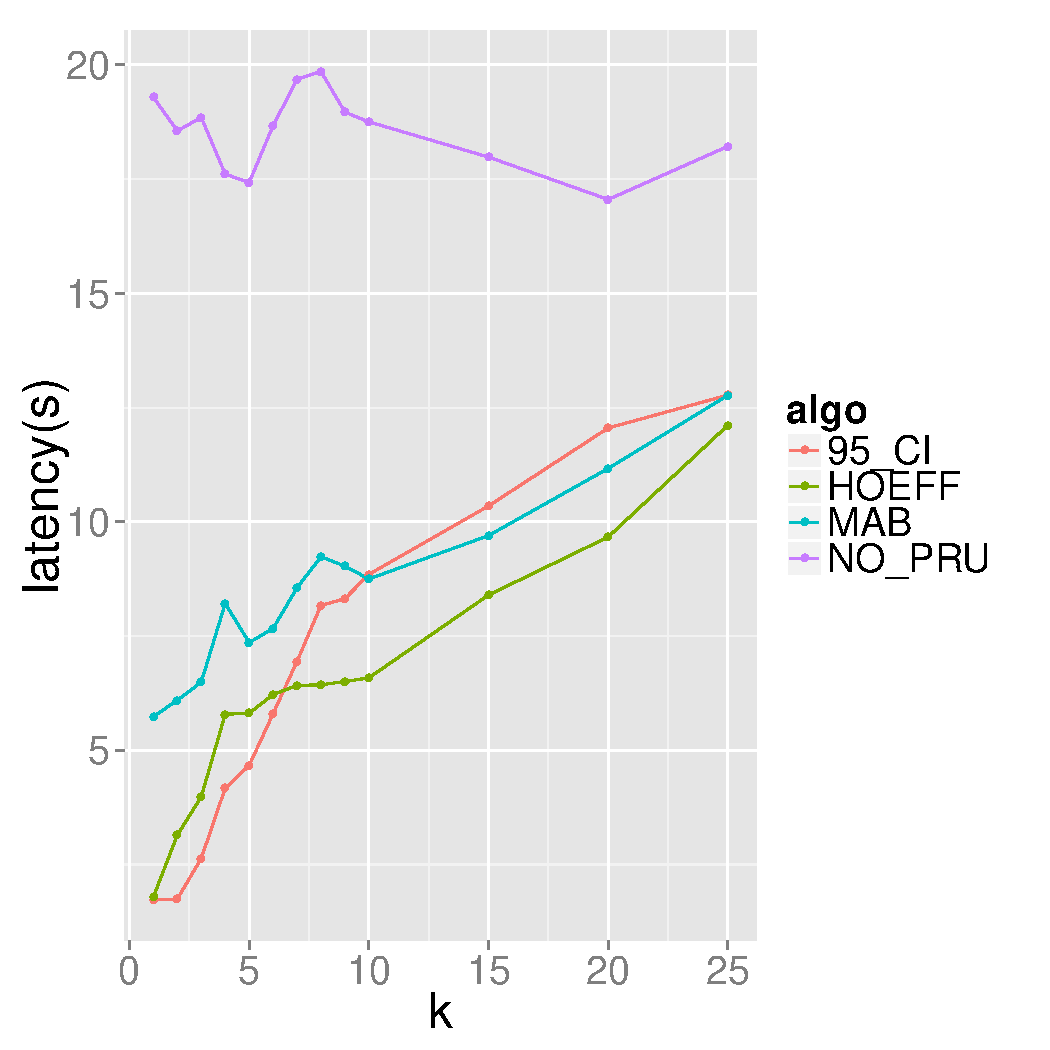
\includegraphics[width=4.2cm] {Images/dia_in_memory_latency.pdf}}
% \caption{Diabetes dataset: latency}
% \label{fig:diabetes_latency}
% \end{subfigure}
% \label{fig:accuracy}
% \caption{Latency for strategies}
% \end{figure}

% \stitle{Accuracy vs.~Latency:}
% {\em \underline{Summary:} Tuning the knobs in the pruning strategies
% gives us further reduction in latency for some losses in accuracy.}
% All of our strategies have ``knobs'' we can use to study the
% trade-off between accuracy and latency: for MAB, this corresponds to the
% number of phases used during processing while for the CI pruning, it 
% corresponds to the size of confidence intervals.
% As expected, if we set these respective parameters to favor greater accuracy 
% (i.e. fewer pruning phases in MAB or larger confidence intervals in CI pruning),
% it also leads to larger latency since fewer views can be pruned at any step.

% Here, we study the impact of these knobs on MAB and 95\_CI, which represent
% two extremes in our set of pruning strategies.
% For MAB, the knob is the number of phases involved in
% processing file; since MAB reduces the number of 
% views by 1 after each phase, the number of
% phases is proportional to the pruning power of our algorithm.
% A large number of phases means that MAB will prune more views and will prune
% them more often.
% Figure \ref{fig:latency_vs_accuracy_mab} shows how latency and accuracy both
% reduce as we increase the number of phases in MAB ($k$=15).
% Each point on the chart corresponds to a different setting for the number of
% phases uses in that implementation of the MAB strategy.
% For 95\_CI, we can vary the $z$-score used
% to determine the size of our confidence intervals.
% That is, we can decide to take a 50\% confidence interval or a 80\% interval or
% a 95\% interval.
% If we take a smaller confidence interval, we will have higher pruning and
% therefore lower latency.
% However, a smaller confidence interval also leads to lower latency since we
% prune views with lower confidence.
% Figure \ref{fig:latency_vs_accuracy_ci} shows that as the $z$-score of the
% confidence interval increases, the accuracy of our strategies increases, but so
% does its latency ($k$=15).
% Every point corresponds to a different size of the confidence intervals.

% \begin{figure}[h] 
% \centering
% \vspace{-10pt}
% \begin{subfigure}{0.49\linewidth}
% \centering
% {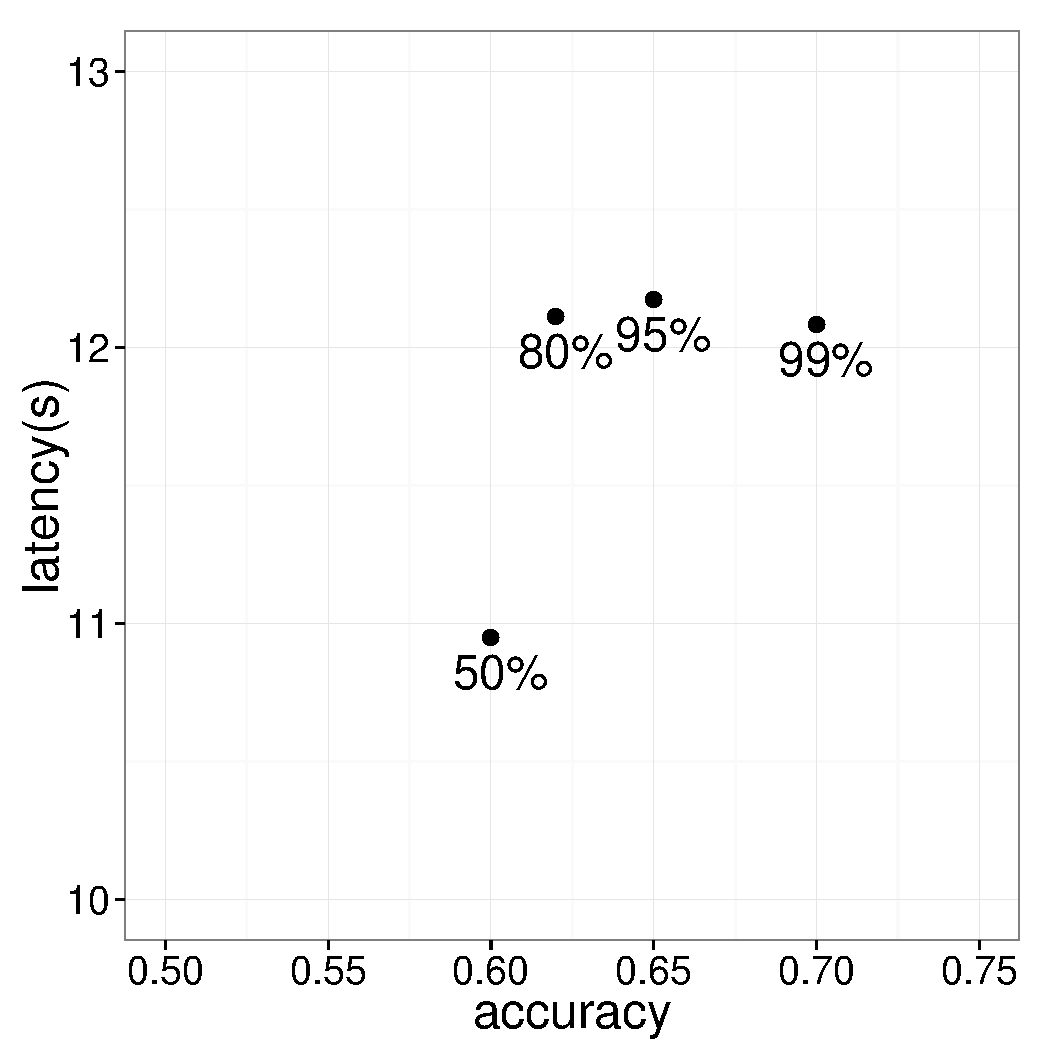
\includegraphics[width=4.2cm] {Images/latency_vs_accuracy_ci.pdf}}
% \caption{95\_CI: Values depict CI \%}
% \label{fig:latency_vs_accuracy_ci}
% \end{subfigure}
% \begin{subfigure}{0.49\linewidth}
% \centering
% {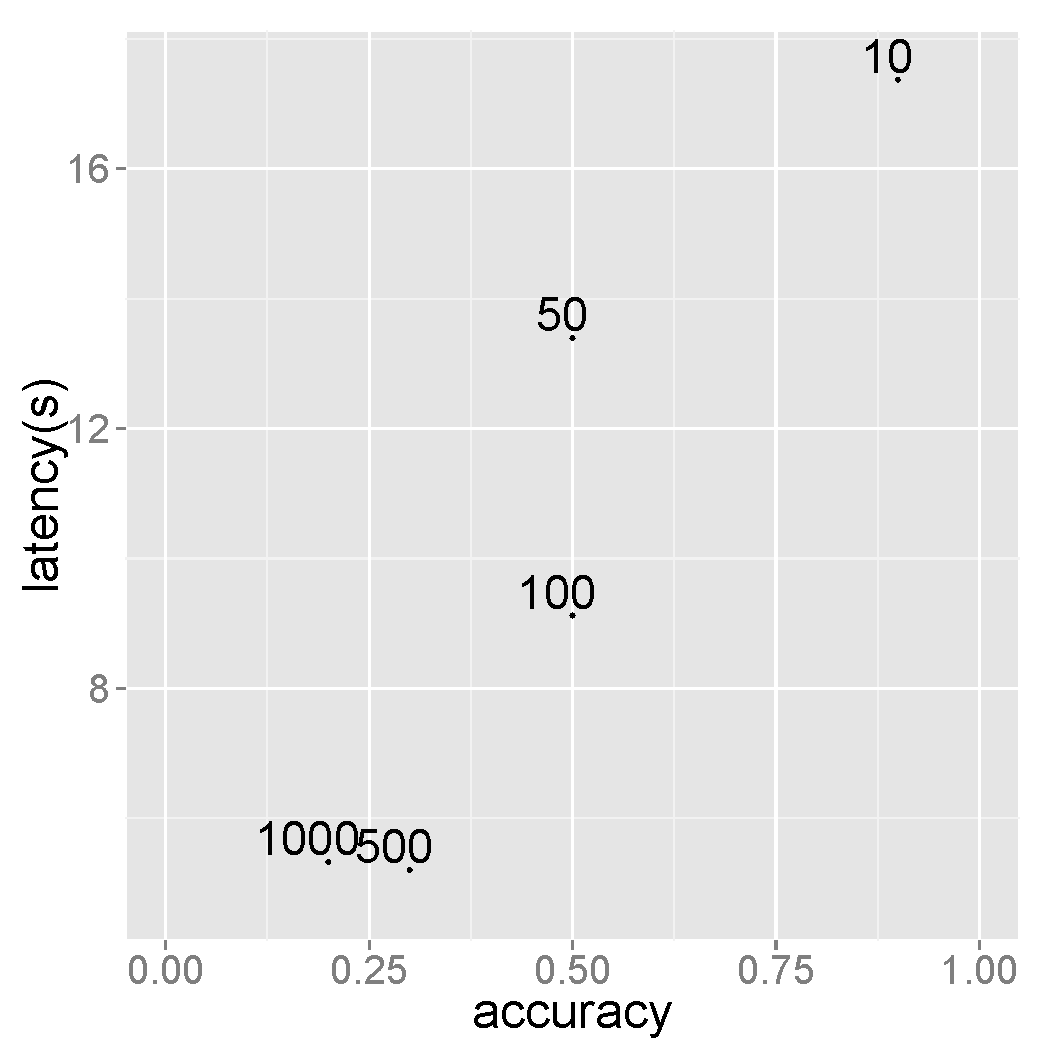
\includegraphics[width=4.2cm] {Images/latency_vs_accuracy_mab.pdf}}
% \caption{MAB: Values depict no. of phases}
% \label{fig:latency_vs_accuracy_mab}
% \end{subfigure}
% \label{fig:accuracy}
% \vspace{-10pt}
% \caption{Latency vs. Accuracy for different strategies}
% \vspace{-20pt}
% \end{figure}









